\chapter{Hardware Layer}
\label{chap:hardware}
While network-based resource disaggregation has gained attention due to advancements in network bandwidth (\S\ref{sec:os}), the inherent latency, limited by the speed of light, still imposes significant overheads. This section explores the potential of next-generation interconnects and their impact on resource disaggregation.

\section{Next-generation Interconnects}

Recent advancements in hardware have led to the development of new-generation interconnects by major hardware vendors, such as NVLink~\cite{nvlink} from Nvidia and Compute Express Link (CXL)~\cite{cxl} from Intel. CXL, in particular, has been introduced as a promising solution to expand memory capacity and bandwidth by attaching external memory devices to PCIe slots, offering a dynamic and heterogeneous computing environment.

\paragraphb{Compute Express Link (CXL)}
As depicted in Figure~\ref{fig:cxl}, CXL encompasses three key protocols: CXL.mem, CXL.cache, and CXL.io. CXL.io serves as the PCIe physical layer. CXL.mem enables processors to access memory over PCIe, while CXL.cache facilitates coherent memory access between processors and accelerators. These protocols allow for the construction of various CXL device types. The initial CXL 1.1 version serves as a memory expander for a single server. Subsequent versions, like CXL 2.0, extend this capability to multiple servers, incorporating CXL switches that coordinate access from different servers and enable various compute nodes to share a large memory pool. The forthcoming CXL 3.0 aims to scale up further, with cache coherency managed by hardware.

Despite extensive research on CXL~\cite{cxl_azure,cxlcentric,demystify}, practical, commercial CXL hardware implementations remain in development, posing challenges in fully understanding performance and system support design for such hardware. Most studies have relied on simulations or FPGA-based CXL hardware~\cite{demystify,intelfpga}, lacking empirical evaluations on ASIC-based CXL hardware. Moreover, existing research often focuses on single aspects of CXL, like capacity or bandwidth, using synthetic benchmarks and neglecting a comprehensive evaluation that includes cost considerations. To gauge the performance of real CXL hardware and assess its suitability for resource disaggregation, we evaluated the latest hardware available: Intel's $\text{4}^{th}$ generation scalable processor (Sapphire Rapids) and Asteralabs's CXL 1.1 memory expander (Type-3 device). Using Intel Memory Latency Checker (MLC)\cite{mlc}, we measured the latency of reading data from the CXL device and local memory equipped with the same amount of DDR5 channels for local and cross-socket access. Figure\ref{fig:cxlperformance} reveals that the latest CXL hardware exhibits a latency of more than $2.5\times$ higher than local memory. However, this gap narrows for cross-socket access, suggesting CXL as another memory tier. This raises questions about whether and how this information should be exposed to applications. Previous research~\cite{tpp} has investigated promoting hot pages from slower-tiered memory at the kernel level to enhance performance while maintaining application transparency.

This study represents the first available evaluation of real CXL 1.1 ASICs. The performance of CXL 2.0 and 3.0 remains to be explored in future work.



\section{Introduction}
\label{sec:intro}

In an age marked by the surge of memory-intensive applications, such as machine learning tasks and High-Performance Computing (HPC) applications, there is an urgent need for expanding the memory capacity and bandwidth~\cite{dataintensive, FlatFlash, cxl-ssd}. 
For instance, a machine learning application with $175$ B model requires $700$ GB of memory to hold its parameters only, not to mention memory requirements for intermediate results and others. That is, the memory requirements of modern applications could easily exceed the memory capability of a single machine due to physical constraints, such as availability of DDR DIMM slots and thermal issues, as well as cost considerations of employing high-density DIMMs~\cite{FlatFlash, cxl-ssd}.

To meet such urgent demands, Compute Express Link (CXL)~\cite{cxl, cxl_azure, cxl-ssd, cxlcentric} is introduced as a groundbreaking interconnect technology. 
CXL promises significant expansion of memory capacity and bandwidth by attaching external memory devices (e.g., DRAM, Flash or persistent memory) to PCIe slots.  
Unlike its predecessors, CXL enables a more dynamic and heterogeneous computing environment, leading to various design trade-offs for performance and cost gains. Commercially debuting with version 1.1, CXL allows direct attachment of external memory devices to the host machine, enabling a unified and coherent memory address space. In such configuration, CXL is predominantly used as a way of memory expansion.
For example, AsteraLabs' A1000~\cite{A1000} CXL memory expansion card supports up to $4$xDDR5 RDIMMs, enabling up to $2$ TB of additional memory for a single server.

%\yupeng{Explicity mention we are focusing in 1.1 here}
\begin{figure}[t]
    \centering
      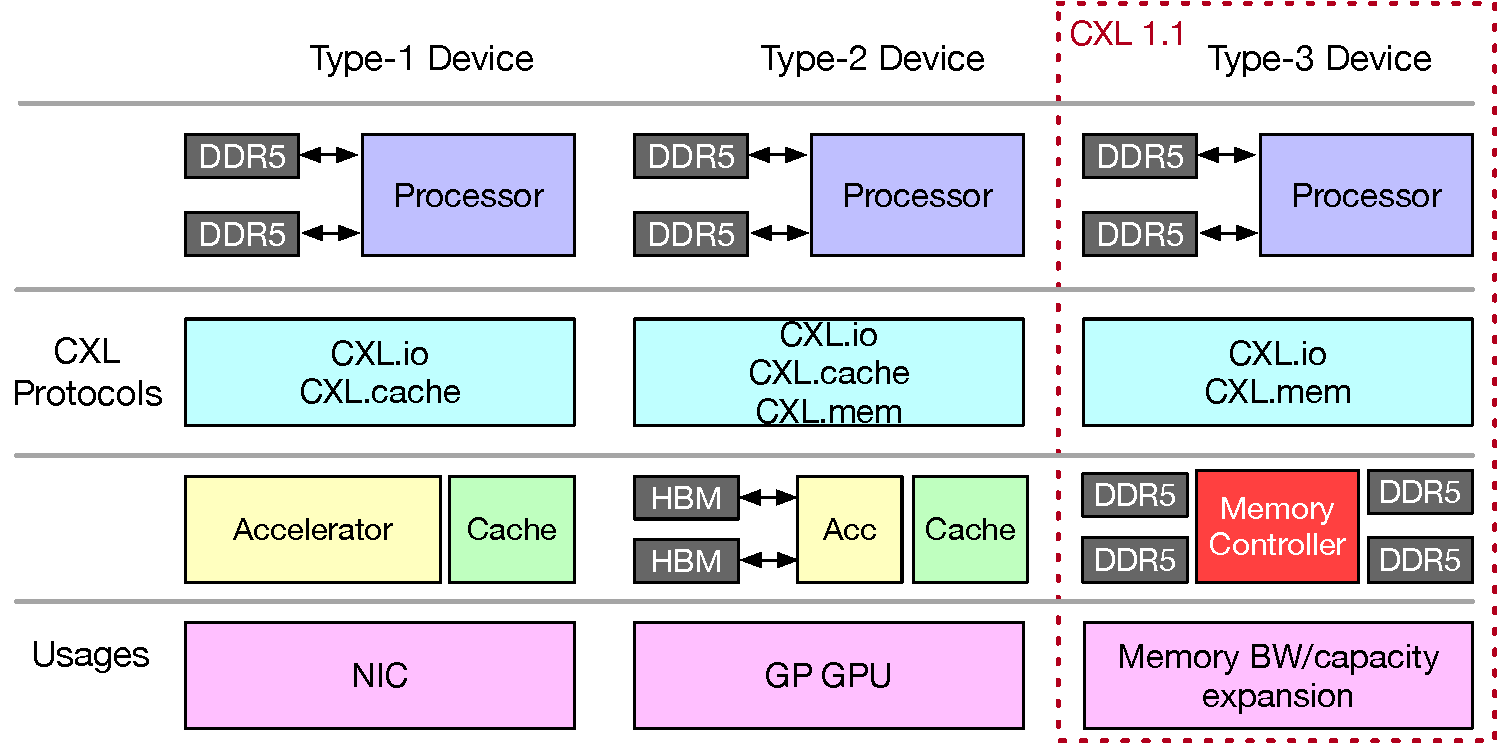
\includegraphics[width=\columnwidth]{fig/cxl/cxl.pdf}
      \vspace{-1.5em}
      \caption[CXL Overview]{\textbf{CXL Overview.} In this study, we focus on commercial CXL 1.1 Type-3 devices, leveraging CXL.io and CXL.mem protocols for memory expansion in single-server environments.} 
    \label{fig:cxl1.1} \vspace{-1.5em}
    \end{figure}

%\yupeng{Correct the claim as the first to explore CXL}
Although substantial studies on CXL memory have been performed in the past~\cite{cxl_azure, cxlcentric, pond, tpp, cxltradeoff,demystify,directcxl, cxl-ssd}, there remains a significant gap of employing these studies to guide the integration of CXL practically.
In particular, we observe the following issues:
(1) Much of the current literature has focused on evaluating CXL hardware through simulations~\cite{pond, cxlcentric} or using FPGA-based setups~\cite{demystify, directcxl}. Although a limited number of studies have begun to assess the raw performance of ASIC-based CXL hardware~\cite{demystify, smt}, there remains a gap in understanding how different system configurations influence the performance of data center applications using CXL memory. Furthermore, the specific applications that could substantially benefit from CXL memory expansion are not yet fully identified.
% on the real performance characteristics of the CXL technique on
(2) While existing studies have begun to explore the cost implications of employing CXL technology, such as the work on memory pooling cost models presented in \cite{CXLPoolCost}, a critical gap remains in understanding the cost-effectiveness of migrating particular types of applications or services to memory expansions facilitated by CXL.
(3) Given the restricted availability of CXL ASIC hardware, the research community faces a notable scarcity of open-source empirical data. This limitation hinders efforts to fully comprehend the performance capabilities of such hardware or to develop performance models based on empirical evidence. 

Our study aims to fill existing knowledge gaps by conducting detailed evaluations of CXL 1.1 for memory-intensive applications, leading to several \textit{intriguing observations}:
Contrary to the common perception that CXL memory, due to its higher latency, should be considered a separate, slower tier of memory~\cite{pond,tpp}, \textbf{we find that shifting some workloads to CXL memory can significantly enhance performance}, even if local memory's capacity and bandwidth are underutilized. This is because using CXL memory can decrease the overall memory access latency by alleviating bandwidth contention on DDR channels, thereby improving application performance.
From our analysis of application performance, we have formulated an abstract cost model (\S\ref{sec:cost}) that predicts substantial cost savings in practical deployments.

In summary, the major contributions of this paper are:
\begin{itemize}
\item \textbf{Empirical Evaluation of ASIC CXL Hardware}:
Our study comprehensively examines the performance of ASIC-based CXL hardware and system configurations in data center applications, offering insights on optimizing CXL memory utilization.

\item \textbf{Cost-Benefit Analysis}: We undertake a comprehensive cost-benefit analysis and develop an Abstract Cost Model to evaluate how CXL memory could substantially reduce real-world applications' TCO (Total Cost of Ownership).

\item \textbf{Open-source data on CXL ASIC performance}: We open source all data and testing configurations under \url{https://github.com/bytedance/eurosys24-artifacts}.


\end{itemize}

The paper organizes as follows. \S\ref{sec:background} introduces basic information of CXL and 
environment setup for the evaluations. \S\ref{sec:micro} presents basic performance characteristic of CXL memory expansion. \S\ref{sec:capacity} and \S\ref{sec:bandwidth} presents findings and suggestions of using CXL as the expansion of memory capacity and bandwidth on data center workloads. \S\ref{sec:cost}  provides a detailed analysis on the potential cost benefits brought by CXL. \S\ref{sec:discussion} discusses how our insights are applicable to future generations of CXL. \S\ref{sec:related} describes related work, and \S\ref{sec:conclusion} concludes the paper.















\section{Background and Methodology}
\label{sec:background}

This section presents an overview of CXL technology, followed by our experimental setup and methodologies.

\begin{figure*}[t]
    \centering
    \subfigure[CXL Server(socket 0 illustrated here).]{
      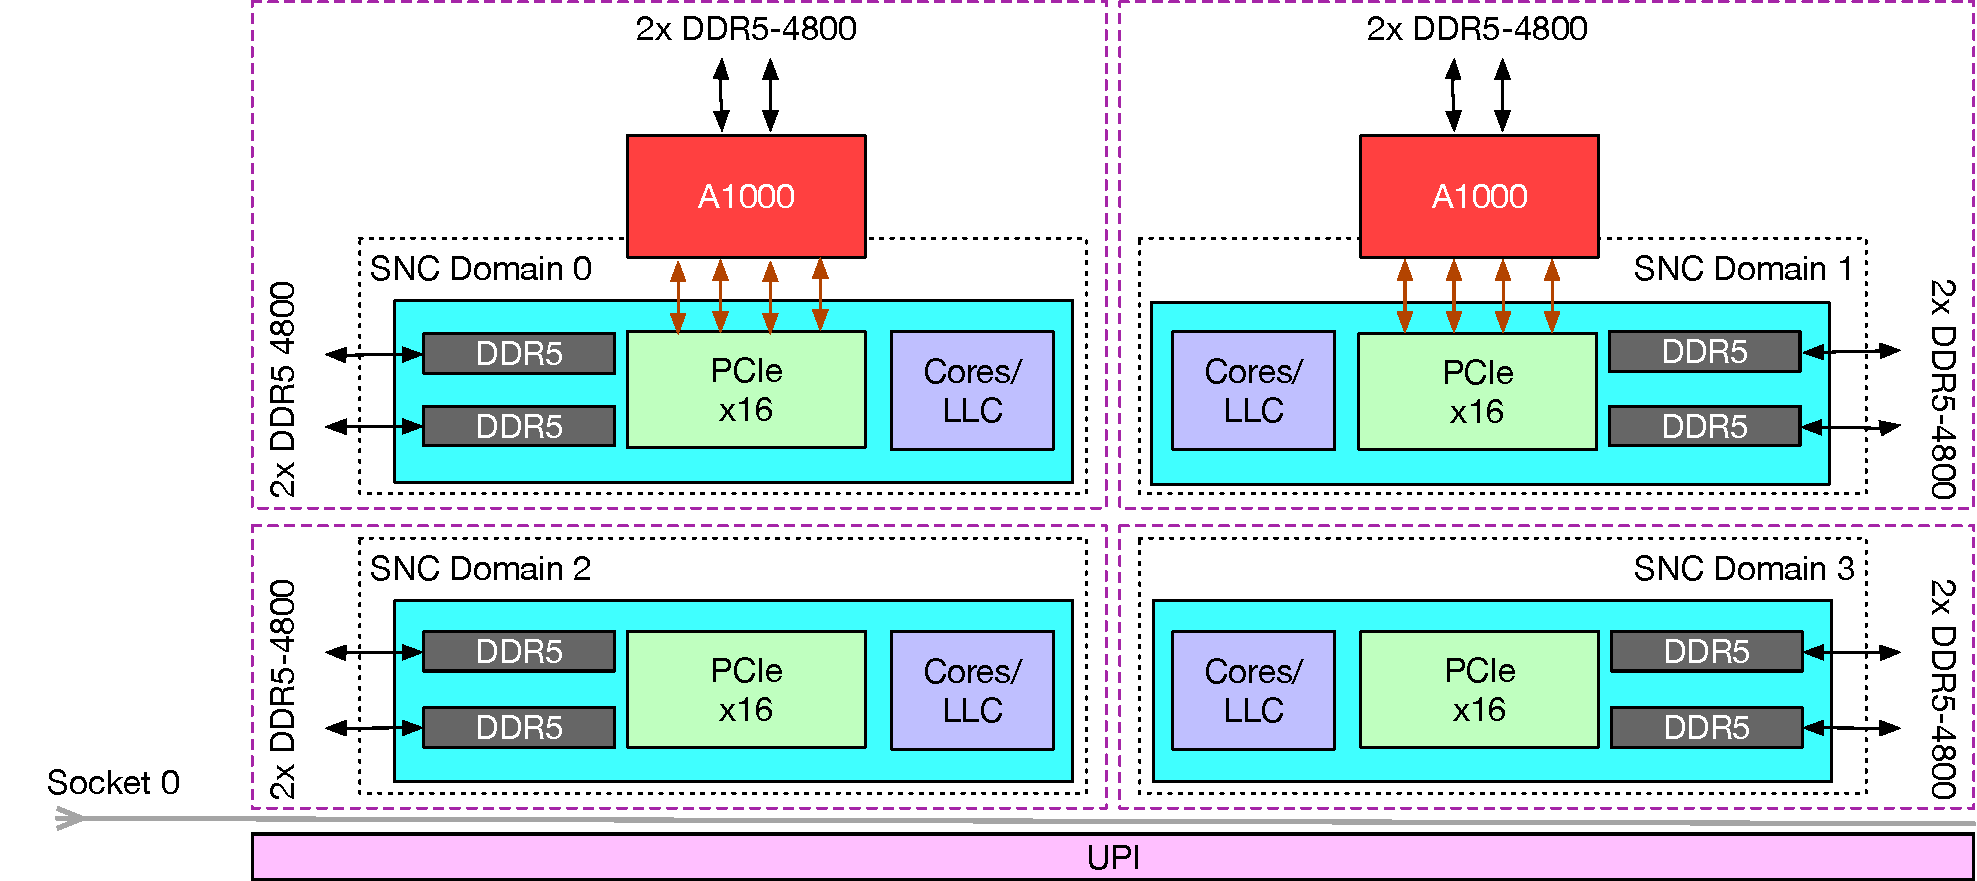
\includegraphics[width=0.60\textwidth]{fig/cxl/server.pdf}
      \label{fig:server}}
    \subfigure[Server setup.]{
      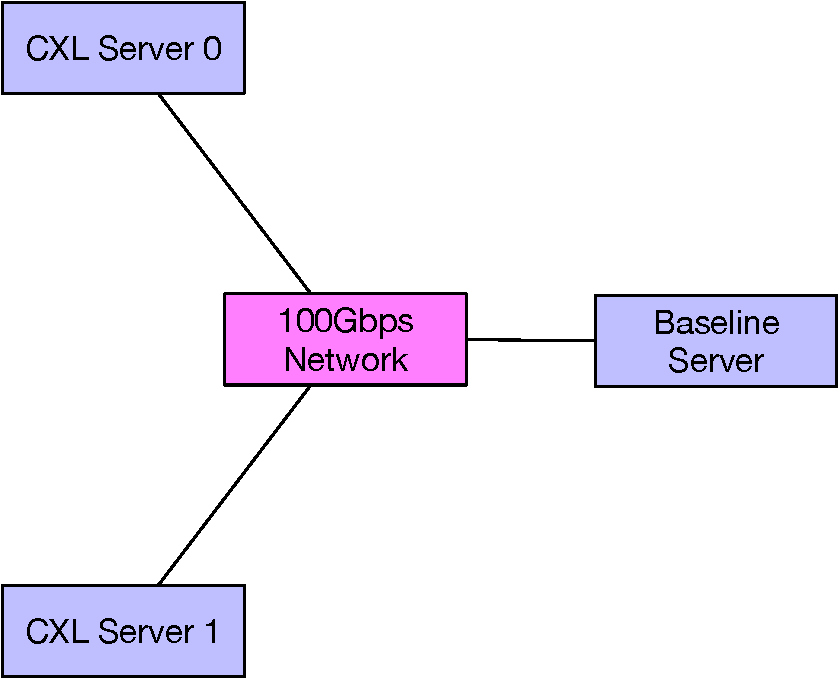
\includegraphics[width=0.33\textwidth]{fig/cxl/platform.pdf}
    \label{fig:platform}}
    \caption[CXL Experimental Platform]{\textbf{CXL Experimental Platform.} (a) Each CXL server is equipped with two A1000 memory expansion cards. SNC-4(\S\ref{ssec:config}) is enabled only for the raw performance benchmarks(\S\ref{sec:micro}) and bandwidth-bound benchmarks(\S\ref{sec:bandwidth}), and each SNC Domain is equipped with two DDR5 channels. (a) illustrates Socket 0; Socket 1 shares a similar setup except for the absence of CXL memory. (b) Our platform comprises two CXL servers and one baseline server. The baseline server replicates the same configuration but lacks any CXL memory cards.}
\end{figure*}

\subsection{Compute Express Link (CXL) Overview}

Compute Express Link (CXL)~\cite{sharma2022compute} is a standardized interconnect technology that facilitates communication between processors and various devices, including accelerators, memory expansion units, and smart I/O devices. CXL is built upon the physical layer of PCI Express® (PCIe®) 5.0~\cite{pcie5.0}, providing native support for x16, x8, and x4 link widths with data rates of $32.0$ GT/s and $64.0$ GT/s. The CXL transaction layer is implemented through three protocols: CXL.io, CXL.cache, and CXL.mem, as depicted in Fig.~\ref{fig:cxl1.1}. \textit{CXL.io} protocol is based on PCIe 5.0 and handles device discovery, configuration, initialization, I/O virtualization, and direct memory access (DMA). \textit{CXL.cache} enables CXL devices to access the host processor's memory. \textit{CXL.mem} allows the host to access memory attached to devices using load/store commands.

CXL devices are categorized into three types, each associated with specific use cases: (1) \textit{Type-1 devices} like SmartNICs utilize CXL.io and CXL.cache for DDR memory communication. (2) \textit{Type-2 devices}, including GPUs, ASICs, and FPGAs, employ CXL.io, CXL.cache, and CXL.mem to share memory with the processor, enhancing various workloads in the same cache domain. (3) \textit{Type-3 devices} leverage CXL.io and CXL.mem for memory expansion and pooling. This allows for increased DRAM capacity, enhanced memory bandwidth, and the addition of persistent memory without sacrificing DRAM slots. Type-3 devices complement DRAM with CXL-enabled solutions, benefiting high-speed, low-latency storage.

%\end{enumerate}

The commercially available version of CXL is 1.1, where a CXL 1.1 device can only serve as a single logical device accessible by one host at a time. Future generations of CXL, like CXL 2.0, are expected to support the partitioning of devices into multiple logical units, enabling up to 16 different hosts to access different portions of memory~\cite{sharma2023introduction}. In this paper, our focus is on commercially available CXL 1.1 Type-3 devices, specifically addressing single-host memory expansion.



\subsection{Hardware Support for CXL}
\label{ssec:cxlhardware}

Recent announcements have introduced CXL 1.1 support for Intel Sapphire Rapids processors (SPR) \cite{SPR} and AMD Zen 4 EPYC "Genoa" and "Bergamo" processors\cite{amdgenoabergamo}. While commercial CXL memory modules are provided by vendors such as Asteralabs~\cite{A1000}, Montage~\cite{mxc}, Micron~\cite{micron}, and Samsung~\cite{smt}, CXL memory expanders are predominantly in prototype stages, with only limited samples available, making access difficult for university labs. Consequently, due to the scarcity of CXL hardware, research into CXL memory has largely depended on NUMA-based emulation~\cite{pond,tpp} and FPGA implementations~\cite{demystify, directcxl}, each with inherent limitations:

\paragraphb{NUMA-based emulation} Given the cache coherent nature and comparable transfer speed of CXL and UPI/xGMI interconnects, NUMA-based emulation~\cite{pond, tpp} is widely adopted to enable fast application performance analysis and software prototyping as the CXL memory is exposed as a remote NUMA node. However, NUMA-based emulation fails to accurately capture the performance characteristics of CXL memory due to differences from CXL and UPI/xGMI interconnects~\cite{cxldatabase}, as shown in previous research~\cite{demystify}.

\paragraphb{FPGA-based implementation} Intel and other hardware vendors use FPGA hardware to implement CXL protocols~\cite{intelfpga}, bypassing the performance inconsistencies of NUMA-based emulation. However, FPGA-based CXL memory falls short in fully utilizing memory chip performance due to its lower operating frequency compared to ASICs~\cite{fpgaasic}. FPGAs prioritize flexibility over performance and are suitable for early-stage CXL memory validation but not production deployment. Intel's recent evaluation~\cite{demystify} uncovered performance issues in FPGA implementations, including reduced memory bandwidth during concurrent thread execution. This hampers rigorous evaluations for memory capacity- and bandwidth-bound applications, which are key use cases for CXL memory expanders. Further discussion on the performance disparity between CXL ASIC and FPGA controllers is in \S\ref{sec:micro}.

To the best of our knowledge, we are one of the pioneers in uncovering the performance characteristics of actual ASIC prototypes designed for CXL memory expansion. The ASIC CXL memory controller we have employed is the A1000~\cite{A1000} developed by AsteraLabs, which implements the CXL interface at speeds of up to 32 GT/s per lane, supporting up to 16 lanes in total. This controller has the capability to accommodate up to 4 DDR5-5600 RDIMM slots, providing a total memory capacity of 2TB.



\subsection{Software Support for CXL}

\label{ssec:cxlsoftware}

While hardware vendors are actively advancing CXL production, a notable deficiency exists in software and OS kernel support for CXL memory. This deficiency has prompted the utilization of specific software enhancements. We summarize the most recent patches in the Linux Kernel that add CXL-aware support, namely: (1) the interleaving policy support (unofficial) and (2) the hot page selection support (official since Linux Kernel v6.1).

\paragraphb{N:M Interleave Policy for Tiered Memory Nodes}

Traditional memory interleave policies distribute data evenly across memory banks, often using a 1:1 ratio. However, the advent of tiered memory systems, which feature CPU-less memory nodes with diverse performance traits, demands more nuanced strategies for optimizing memory bandwidth, especially for bandwidth-heavy applications. The interleave patch~\cite{Interleavepatch} introduces an innovative N:M interleave policy to address this, allowing for an allocation scheme where N pages are directed to high-performance (top-tier) nodes and M pages to lower-tier nodes. For example, using a 4:1 ratio directs $80\%$ of traffic to top-tier nodes and $20\%$ to low-tier nodes, adjustable through the \texttt{vm.numa\_tier\_interleave} parameter. While the patch showcases compelling evaluation results~\cite{Interleavepatch}, it's crucial to note that optimal memory distribution depends on specific hardware and application characteristics. Given the higher latency of CXL memory, as demonstrated in \S\ref{sec:micro}, performance-sensitive applications should undergo thorough profiling and benchmarking to maximize the advantages of interleaving and mitigate potential performance trade-offs.


\paragraphb{NUMA Balancing \& Hot Page Selection}

The memory subsystem, now termed a memory tiering system, accommodates various memory types like PMEM and CXL Memory, each with differing performance characteristics. To optimize system performance, "hot pages" (frequently accessed) should reside in faster memory tiers like DRAM, while "cold pages" (less frequently accessed) should be in slower tiers like CXL memory. Recent Linux Kernel patches address this:

1. The \textit{NUMA-balancing} patch~\cite{numaautobalancing} uses a latency-aware page migration strategy, focusing on promoting recently accessed pages (MRU). It scans NUMA balancing page tables and hints page faults. However, it may not accurately identify high-demand pages due to extended scanning intervals, potentially causing latency issues for some workloads.

2. The \textit{Hot Page Selection} patch"~\cite{hot} introduces a Page Promotion Rate Limit (RPRL) mechanism to control the rate of page promotions and demotions. While this extends promotion/demotion times, it improves workload latency. The hot page threshold is dynamically adjusted to align with the promotion rate limit.

Additionally, research prototypes like TPP~\cite{tpp} share a similar concept with optimizations and are being considered for integration into the Linux Kernel~\cite{tpppatch}. However, we faced challenges with TPP when running memory-bandwidth-intensive applications, resulting in unexplained performance degradation. Hence, we rely on the well-tested kernel patches integrated into Linux Kernel since version $6.1$.







\subsection{Experimental Platform Description}
The evaluation testbed, as illustrated in Fig. \ref{fig:platform}, consists of three servers. Two of these servers are designated as CXL experiment servers. Each of these servers is equipped with dual Intel Xeon 4th Generation CPUs (Sapphire Rapids, or SPR), $1$ TB of $4800$ MHz DDR5 memory, two $1.92$ TB SSDs, and a pair of A1000 CXL Gen5 x16 ASIC memory expanders modules from AsteraLabs, each with $256$ GB of 4800MHz memory (resulting in a total of $512$ GB memory per server). Both A1000 memory modules are attached to socket $0$. The third server serves as the baseline and is configured identically to the CXL experiment servers, except for the absence of the CXL memory expanders. It is designated for initiating client requests and running workloads that strictly utilize the main memory during the application assessments. All servers are interconnected via $100$ Gbps Ethernet links.









\section{CXL 1.1 Performance Characteristics}
%\yupeng{Check the absolute value of each number}
\label{sec:micro}


In this section, we assess the performance of the CXL memory expander and compare it directly with main memory, which we designate as \textbf{MMEM} for clarity against CXL memory. We analyze workload patterns and evaluate performance differences between local and remote socket scenarios.

\begin{figure}[t]
\centering
 \vspace{-0.2em}
\subfigure[Local-socket MMEM]{
  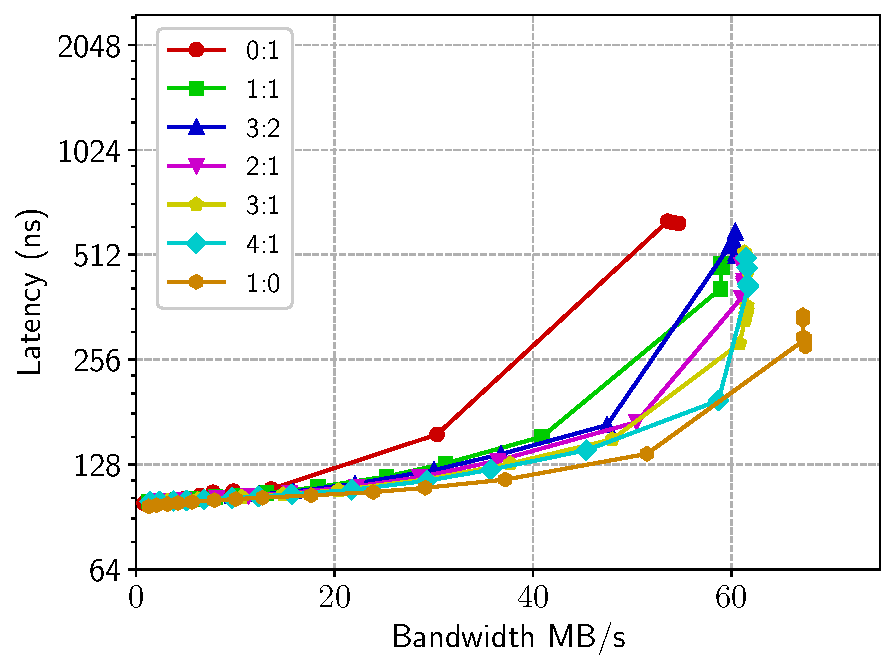
\includegraphics[width=0.24\textwidth]{fig/cxl/cxl_dram_workload_rw_c16_r0.pdf}
  \label{fig:localdram}}%
\subfigure[Remote-socket MMEM]{
  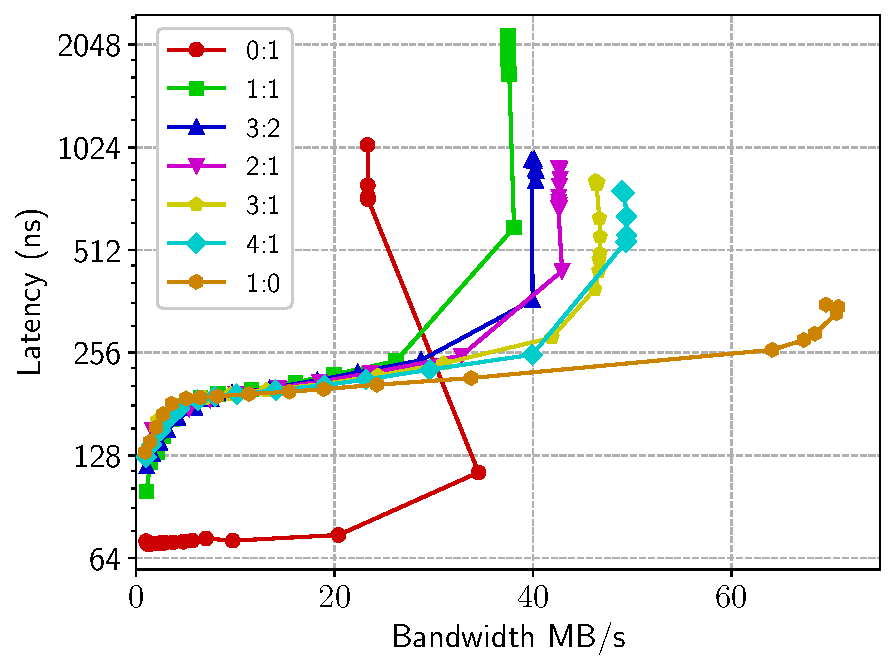
\includegraphics[width=0.24\textwidth]{fig/cxl/cxl_dram_workload_rw_c16_r0_rs.pdf}
  \label{fig:remotesocketdram}}% 
\subfigure[Local-socket CXL]{
  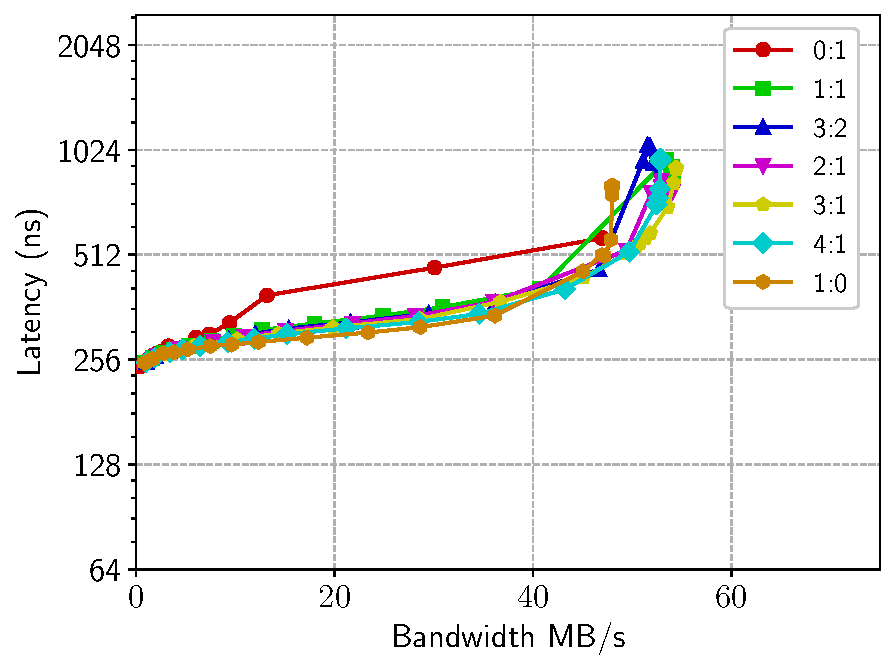
\includegraphics[width=0.24\textwidth]{fig/cxl/cxl_cxl_workload_rw_c16_r0.pdf}
  \label{fig:cxllocalsocket}}%
  \subfigure[Remote-socket CXL]{
  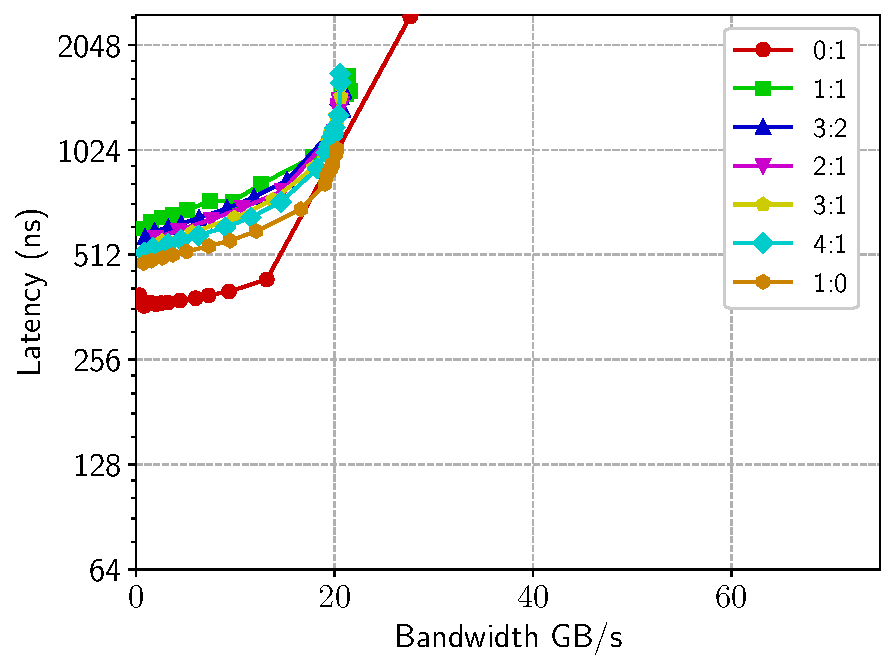
\includegraphics[width=0.24\textwidth]{fig/cxl/cxl_cxl_workload_rw_c16_r0_rs.pdf}
  \label{fig:cxlremotesocket}}%
 \caption[Overall effect of read-write ratio on MMEM and CXL across different distances]{\textbf{Overall effect of read-write ratio on MMEM and CXL across different distances.} The workloads are represented by read:write ratios (e.g., $0$:$1$ for write-only, $1$:$0$ for read-only). Accessing CXL memory locally incurs higher latency compared to MMEM but is more comparable to accessing MMEM on a remote socket. MMEM bandwidth peaks at $67$ GB/s, versus $54.6$ GB/s for CXL memory. Performance significantly declines when accessing CXL memory on a remote socket (\S\ref{ssec:performance}).  In specific scenarios, such as the write-only workload ($0$:$1$) in (b), the plot may show instances where bandwidth decreases and latency increases with heavier loads. The Y-axis is on a logarithmic scale.}
\label{fig:microbench-1}
\end{figure}

\begin{figure*}[t]
\centering
 \vspace{-0.2em}
  \subfigure[Read-only workload]{
  % include first image
  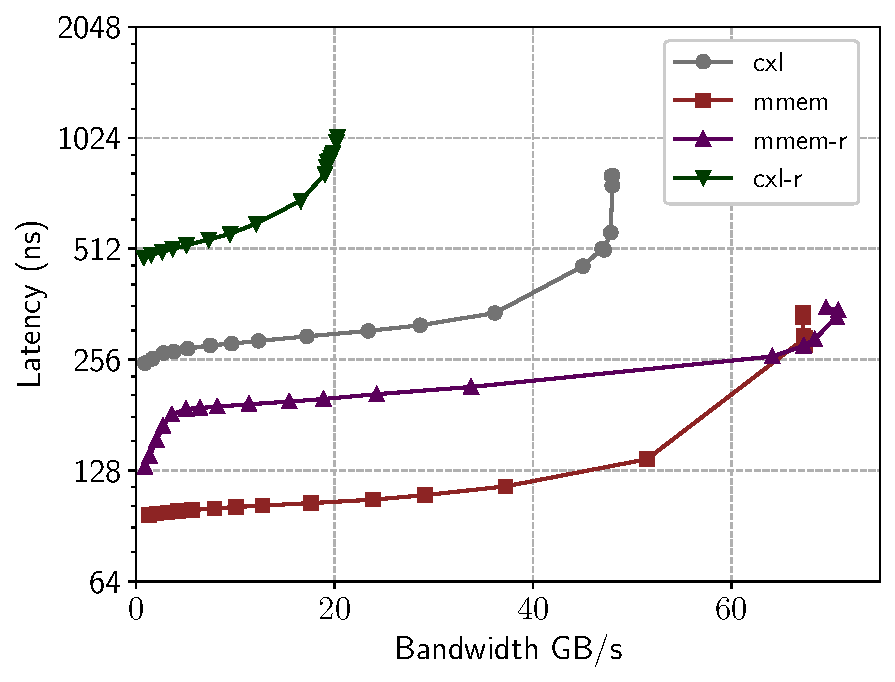
\includegraphics[width=0.24\textwidth]{fig/cxl/cxl_mix_workload0_c16_r0.pdf}
  \label{fig:readonly}}%
    \subfigure[Read:Write = $4$:$1$ workload]{
  % include first image
  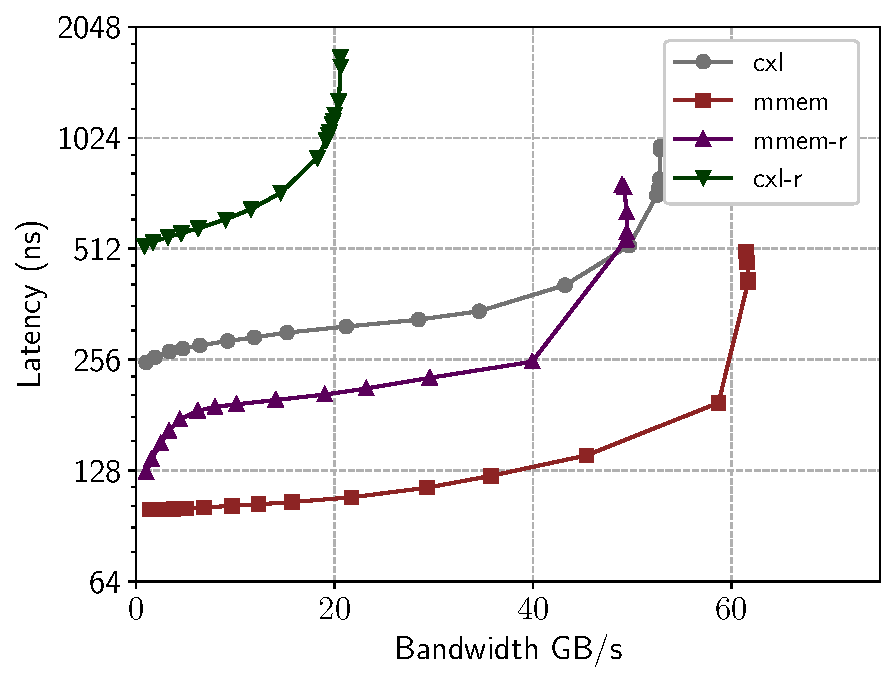
\includegraphics[width=0.24\textwidth]{fig/cxl/cxl_mix_workload12_c16_r0.pdf}
  \label{fig:readwrite41}}%
  \subfigure[Read:Write = $3$:$1$ workload]{
  % include first image
  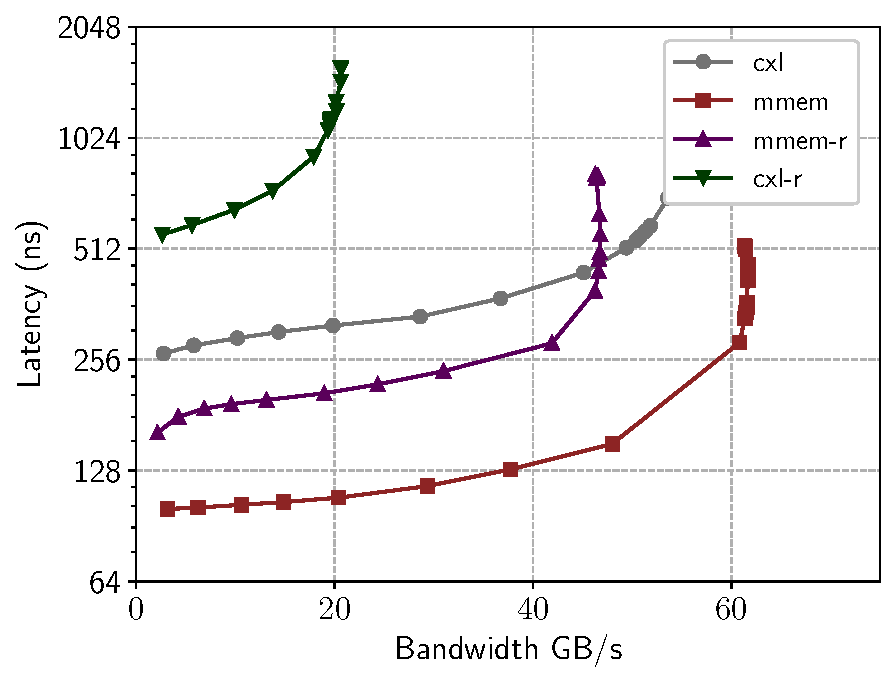
\includegraphics[width=0.24\textwidth]{fig/cxl/cxl_mix_workload3_c16_r0.pdf}
  \label{fig:readwrite31}}%
  \subfigure[Read:Write = $2$:$1$ workload]{
  % include first image
  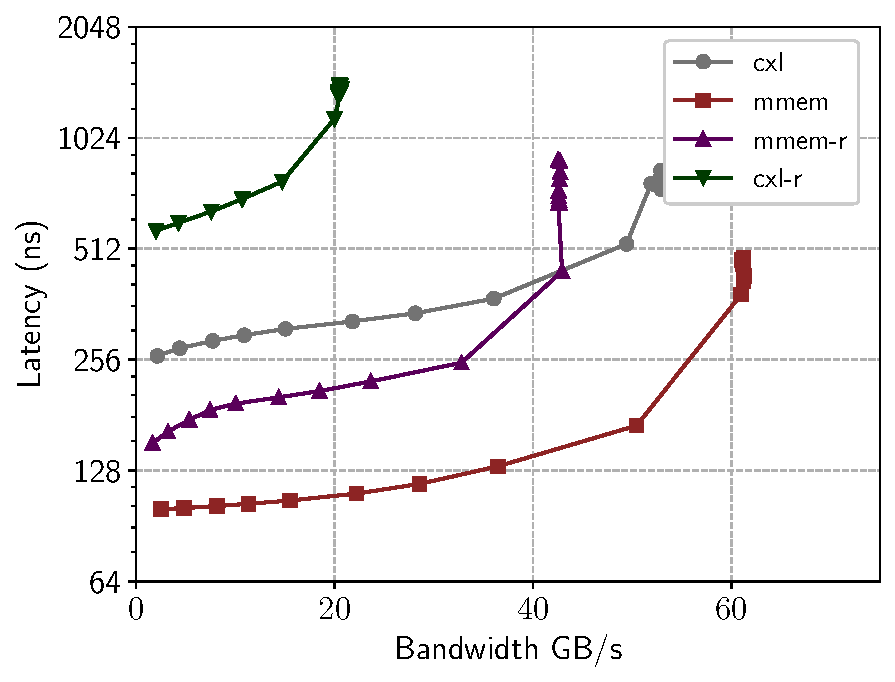
\includegraphics[width=0.24\textwidth]{fig/cxl/cxl_mix_workload2_c16_r0.pdf}
  \label{fig:readwrite21}}%
  \\
  \subfigure[Read:Write = $1$:$1$ workload]{
  % include first image
  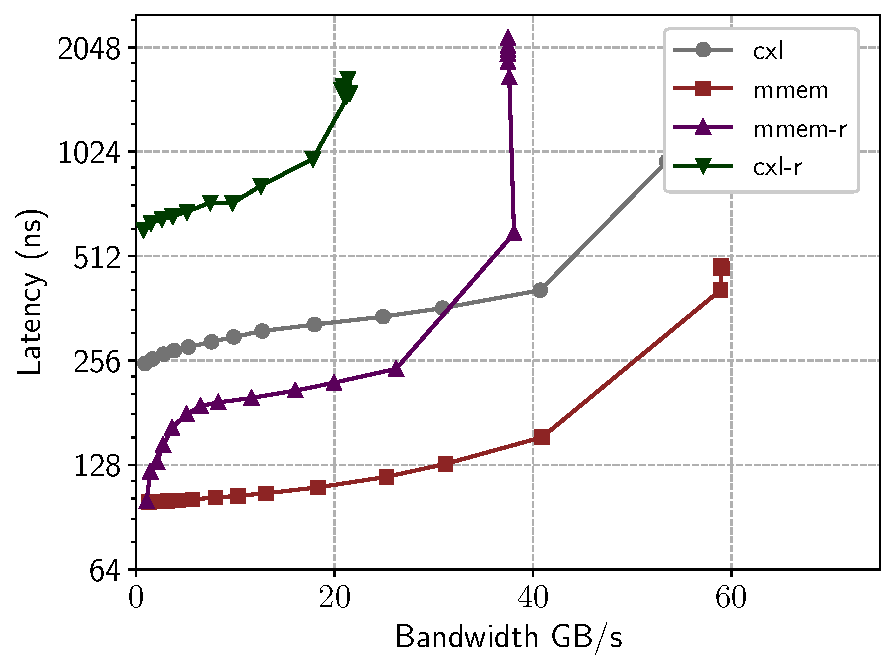
\includegraphics[width=0.24\textwidth]{fig/cxl/cxl_mix_workload5_c16_r0.pdf}
  \label{fig:readwrite11}}%
  \subfigure[Write-only workload]{
  % include first image
  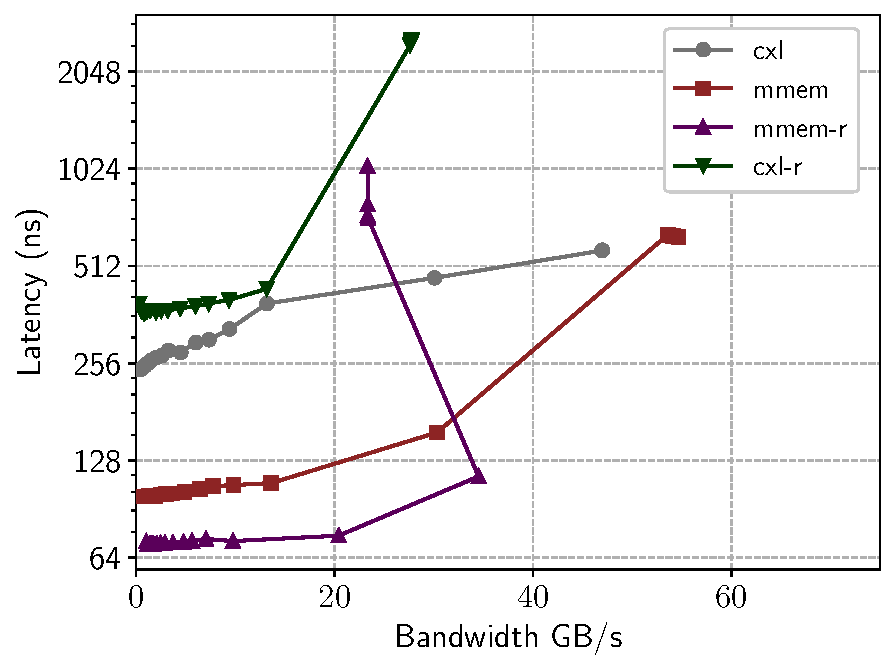
\includegraphics[width=0.24\textwidth]{fig/cxl/cxl_mix_workload6_c16_r0.pdf}
  \label{fig:writeonly}}%
  \subfigure[Read-only workload (random)]{
  % include first image
  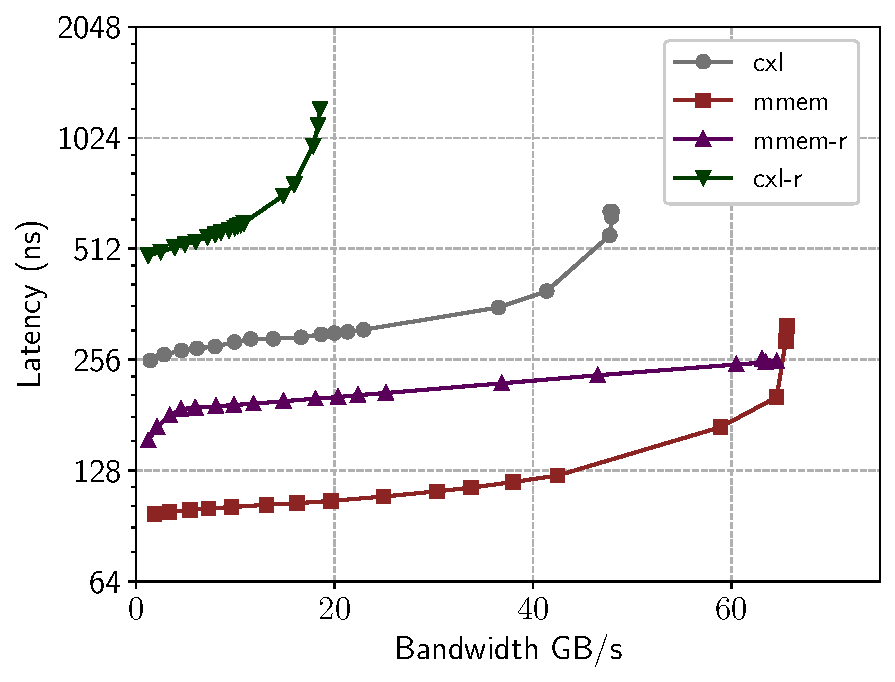
\includegraphics[width=0.24\textwidth]{fig/cxl/cxl_mix_workload0_c16_r1.pdf}
  \label{fig:readdatasize}}%
    \subfigure[Write-only workload (random)]{
  % include first image
  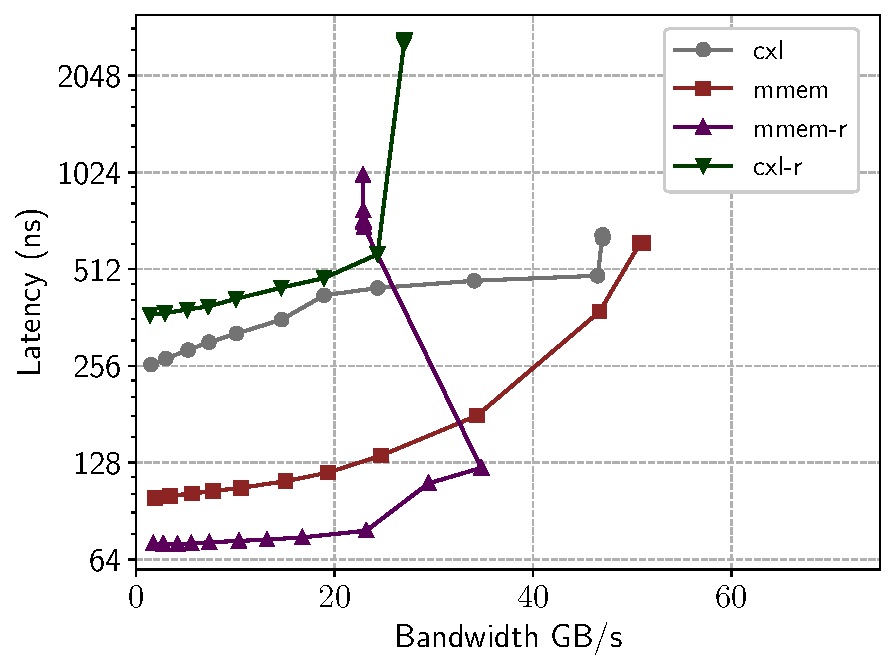
\includegraphics[width=0.24\textwidth]{fig/cxl/cxl_mix_workload6_c16_r1.pdf}
  \label{fig:writedatasize}}%
 \caption[A detailed comparison of MMEM versus CXL over diverse NUMA/socket distances and workloads]{\textbf{A detailed comparison of MMEM versus CXL over diverse NUMA/socket distances and workloads.} (a)-(f) shows the latency-bandwidth trend difference of accessing data from different distances in sequential access pattern, sorted by the proportion of write. We refer to main memory as \textbf{MMEM}, with MMEM-r and CXL-r representing remote socket MMEM and cxl memory access, respectively. The Y-axis is on a logarithmic scale.}
\label{fig:microbench-2}
\end{figure*}

\subsection{Experimental Configuration}
\label{ssec:config}
For each dual-channel A1000 ASIC CXL memory expander~\cite{A1000}, we connect two DDR5-4800 memory channels, achieving a total capacity of $256$ GB. To provide a fair comparison between MMEM and CXL-attached DDR5 memory, we utilize the Sub-NUMA Clustering (SNC)~\cite{snc} feature to ensure the number of memory channels is the same in both settings. 
%\yupeng{Sub NUMA clustering usage in later sections}

\paragraphb{Sub-NUMA Clustering(SNC)} Sub-NUMA Clustering (SNC) serves as an enhancement over the traditional NUMA architecture. It decomposes a single NUMA node into multiple smaller semi-independent sub-nodes (domains). Each sub-NUMA node possesses its own dedicated local memory, L3 caches, and CPU cores. In our experimental setup (Fig. ~\ref{fig:server}), we partition each CPU into four sub-NUMA nodes. Each sub-NUMA node is equipped with two DDR5 memory channels connected to two $64$ GB DDR5-4800 DIMMs. Enabling SNC requires setting the IMC (Integrated Memory Controllers) to 1-way interleaving. According to the specifications, a single DDR5-4800 channel has a theoretical peak bandwidth of $38.4$ GB/s~\cite{cxlcentric}. Therefore, each sub-NUMA node has a combined memory bandwidth of up to $76.8$ GB/s.

\paragraphb{Intel Memory Latency Checker (MLC)} We leverage Intel's Memory Latency Checker (MLC) to examine loaded-latency for various read-write workloads, adopting a $64$-byte access size same as prior work~\cite{demystify}. We deploy $16$ MLC threads, and it's important to note that while the thread count is a configurable parameter in MLC, it doesn't directly dictate memory request concurrency. MLC assigns separate memory segments for each thread to access simultaneously. Specifically, when evaluating loaded latency, MLC incrementally increases the operation rate of each thread. Our findings indicate that employing $16$ threads with MLC precisely measures both the idle and loaded latency and the point at which bandwidth becomes saturated. MLC accommodates a broad spectrum of workloads including those with varied read-write mixes and non-temporal writes.

Our study is focused on addressing the following research questions:

\begin{itemize}
    \item How is the performance of the CXL-attached memory compared to that of local-socket/remote-socket main memory?
    \item What is the performance impact of the CXL memory under different read-write ratios and access patterns (random vs. sequential)?
    \item How do main memory and CXL memory behave under high memory load conditions?
\end{itemize}


\subsection{Basic Latency and Bandwidth Characteristics}
\label{ssec:performance}
This section outlines our findings on memory access latency and bandwidth for different memory configurations: local-socket main memory (MMEM), remote-socket main memory (MMEM-r), CXL memory (CXL), and remote-socket CXL memory (CXL-r). Figure \ref{fig:localdram} shows the loaded latency curve for MMEM under varied read-write mixes. The read-only workload hits a peak bandwidth of roughly $67$ GB/s, reaching $87\%$ of its theoretical maximum. Yet, as write operations increase, bandwidth dips, with write-only tasks dropping to $54.6$ GB/s. We note an initial memory latency of about $97$ ns, which spikes exponentially as bandwidth nears full capacity, a sign of bandwidth contention~\cite{cxl-centric, mt2}. Interestingly, latency starts to significantly increase at $75\%$-$83\%$ of bandwidth utilization, surpassing prior estimates of $60\%$ from earlier studies~\cite{cxl-centric}.


Figure \ref{fig:remotesocketdram} illustrates the latency differences when accessing MMEM via a remote socket. For read-only tasks, latency begins at approximately $130$ ns, contrasting sharply with just $71.77$ ns for write-only operations. This reduced latency for write-only workloads results from non-temporal writes, which proceed asynchronously without awaiting confirmation. Despite read-only tasks achieving maximum bandwidth comparable to that of local MMEM, incorporating more write operations significantly diminishes bandwidth, attributed to the additional UPI traffic necessitated by cache coherence protocols. Interestingly, the write-only workload generate minimal UPI traffic but suffer the lowest bandwidth as it utilize only one direction of the UPI's bidirectional capabilities. Moreover, latency escalation occurs earlier in remote socket memory accesses than in local ones, primarily due to queue contention at the memory controller.

Fig. ~\ref{fig:cxllocalsocket} illustrates the latency curve for CXL memory expansion, demonstrating a minimum latency of $250.42$ ns. Interestingly, despite additional PCIe and CXL memory controller overhead on the datapath, accessing CXL follows the same "Bandwidth contention" trend as MMEM. The latency of accessing CXL on the same socket remains relatively stable as bandwidth increases, with a maximum bandwidth of around $56.7$ GB/s, achieved when the workload is $2$:$1$ read-write ratio. The reduction in maximum bandwidth compared to DRAM is attributed to PCIe overhead, such as extra headers. The maximum bandwidth for read-only workloads is smaller due to PCIe bi-directionality, preventing full bandwidth utilization. Fig. ~\ref{fig:cxlremotesocket} reveals the latency-bandwidth plot for accessing CXL from a remote socket, incurring an exceptionally high idle latency of $485$ ns. In addition, the maximum memory bandwidth is unexpectedly halved, reaching just $20.4$ GB/s for $2$:$1$ read-write ratio, which is a much more severe performance drop compared to accessing MMEM from the remote NUMA node in Fig. ~\ref{fig:cxlremotesocket}. Since running a read-only towards a CXL Type-3 device on the remote socket does not generate substantial coherence traffic, initial speculation regarding cache coherence is ruled out. Further investigation utilizing the Intel Performance Counter Monitor (PCM)~\cite{pcm} also confirms that the UPI utilization is consistently below $30\%$.
Discussions with Intel suggest this performance bottleneck is likely due to limitations in the Remote Snoop Filter (RSF) on the current CPU platform, anticipated to be addressed in the next-generation processors~\cite{emerald_rapids}.



\subsection{Different Read-Write Ratios \& Access Pattern}

Fig. ~\ref{fig:readonly}-\ref{fig:writeonly} present a performance comparison for a specific workload with varying read-write ratios. The results align with our observation that accessing CXL from a remote socket introduces exceptionally high latency and low bandwidth.
When accessing CXL from the same socket, latency is $2.4$-$2.6$ $\times$ that of local DDR and $1.5$-$1.92$ $\times$ that of remote socket DDR.
This suggests that running applications directly on CXL may significantly drop performance.
However, when workloads span multiple NUMA nodes within the same socket, accessing CXL locally is comparable to accessing remote NUMA node memory.
Additionally, the latency-bandwidth knee-point shifts to the left as the proportion of write operations in the workload increases.
Fig.~\ref{fig:readdatasize} and~\ref{fig:writedatasize} display the results of running both read-only and write-only workloads, utilizing random access patterns instead of sequential access. Notably, we do not observe any significant performance disparities under these conditions.

\subsection{Key insights}
% Based on the experiment above, we summarize our key findings.
\paragraph{Avoiding Remote Socket CXL Access.}
CXL memory expansion is commonly utilized for applications that are demanding in terms of memory, particularly those limited by memory capacity or bandwidth. In such contexts, accessing memory across sockets is not uncommon. It is important for software developers to recognize the potential decline in performance when CXL memory is accessed from a remote socket and to strategize against cross-socket CXL memory accesses in their applications. Additionally, hardware vendors should perform cooperative testing and validation of their products to ensure compatibility between CXL memory modules and the processors' CXL support. With adequate support for the CXL 1.1 protocol, we expect that the maximum bandwidth attainable when accessing CXL memory across sockets could approximate the bandwidth seen when accessing MMEM across sockets.

\paragraph{Bandwidth Contention}
Previous research~\cite{mt2, cxlcentric} has brought attention to issues related to bandwidth contention. We further examine how memory latency varies with varying read-write ratios under bandwidth contention. While latency remains relatively stable at low to moderate bandwidth utilization levels, it increases exponentially as bandwidth approaches higher levels, primarily due to queuing delays in the memory controller~\cite{cxl-centric}. Furthermore, the knee-point in latency shifts to lower memory bandwidth when there is a higher proportion of write operations in the workload. Interestingly, CXL-attached memory has often been characterized by industry and research community as 'tiered memory'~\cite{demystify, tpppatch, Interleavepatch}, suggesting that it serves as a slower and less performant memory layer to be considered only when MMEM is fully utilized.
However, we argue against this simplistic view of CXL-memory. Allocators and kernel-level page placement policies should consider the available bandwidth in MMEM.
Even if a substantial portion of memory bandwidth in MMEM remains unused, e.g., $30\%$, offloading a portion of the workload, e.g., $20\%$, to CXL memory can lead to overall performance improvements. 
Our recommendation is to regard CXL memory as a valuable resource for load balancing, even when local DRAM bandwidth is not fully utilized. Subsequent real-world evaluations support these insights (\S\ref{sec:bandwidth}).

\paragraph{Comparison with FPGA-based CXL implementations.}
Intel recently disclosed latency and bandwidth performance metrics for their FPGA-based CXL prototype~\cite{demystify}. While they provided insights into relative latency and bandwidth efficiency for soft and hard IP implementations, performance under load was not shared. Our measurements indicate that the ASIC CXL solution only introduces a less than $2.5x$ overhead in access latency compared to MMEM, surpassing most of Intel's measurements. However, the FPGA-based solution achieved only $60\%$ of the PCIe bandwidth due to the inefficiency of the memory controller, while the Asteralabs A1000 prototype reached an impressive $73.6\%$ bandwidth efficiency, clearly outperforming Intel's FPGA-based solution.

% !TEX root = ../paper.tex

\section{Memory Capacity-bound Applications}
\label{sec:capacity}


\begin{figure*}[t]
\centering
 %\vspace{-0.2em}
  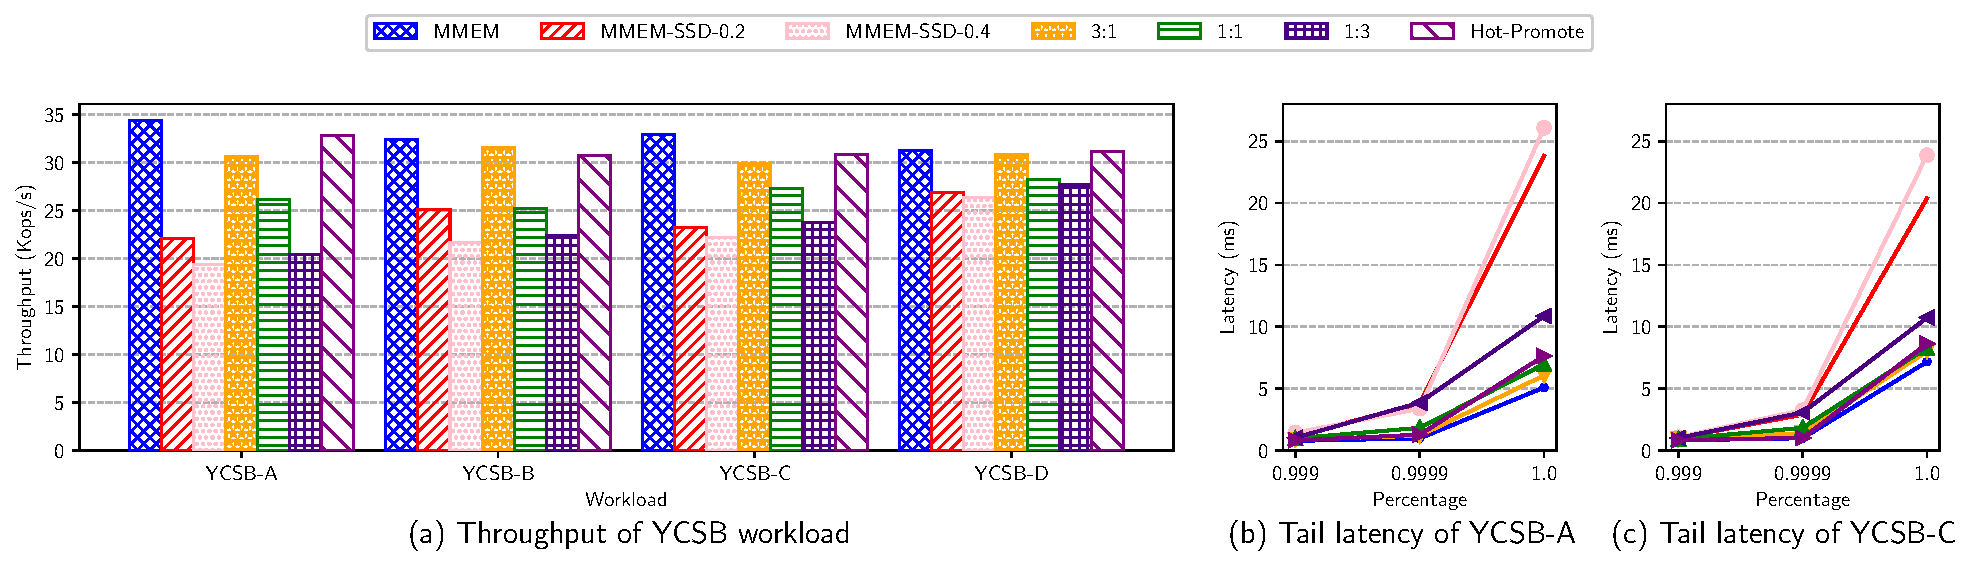
\includegraphics[width=1\textwidth]{fig/cxl/redis_ycsb_cxl.pdf}
  %\vspace{-1.5em}
  \caption[KeyDB YCSB latency and throughput under different configurations]{\textbf{KeyDB YCSB latency and throughput under different configurations.} (a) Average throughput of four YCSB workload under different system configuration. (b) Tail latency of YCSB-A (c) Tail latency CDF of YCSB-C, both reported by the YCSB client~\cite{YCSB}.}
  \label{fig:ycsb_cxl}
\end{figure*}

One of the most significant advantages of integrating CXL memory into modern computing systems is the opportunity for significantly larger memory capacities. To elucidate the potential benefits, we focus on three particular use cases (1) key-value stores, a commonly used application in data centers. (2) Big data analytical application. (3) Elastic computing from cloud providers.

\subsection{In-memory key-value stores}
\label{ssec:keydb}
Redis~\cite{redis} is an open-source in-memory key-value store and one of the most popular NoSQL databases. Redis employs a user-defined parameter, \texttt{maxmemory}, to limit its memory allocation for storing user data. Like traditional memory allocators (e.g., malloc()), Redis may not return memory to the system after key deletion, particularly if deleted keys were on a memory page with active ones. This necessitates memory provisioning based on peak demand, making memory capacity the major bottleneck for Redis deployments~\cite{manageredis} in data centers. Google Cloud suggests keeping memory usage below $80\%$~\cite{googlecloud}, whereas other sources recommend a limit of $75\%$~\cite{manageredis}. 

Due to the substantial infrastructure costs for memory-only deployment, Redis Enterprise~\cite{redisenterprise} is the commercial variant extensively supported by leading cloud platforms (e.g., AWS, Google Cloud, or Azure). It introduces "Auto Tiering"\cite{redisautotiering} to allow data overflow to SSDs, offering an economically viable option for database expansion beyond the limits of RAM capacity. Given that Redis Enterprise is not accessible on our experiment platform, we employ KeyDB as an alternative. KeyDB extends Redis's capabilities by adding KeyDB Flash, which uses RocksDB for persistent storage. The FLASH feature enables all data is written to the disk for persistence, with hot data remaining in memory as well as disk.

\subsubsection{Methodology and Software Configurations.}

In our study, we investigate the performance effects of maximizing memory utilization on a KeyDB server. We deploy a single KeyDB instance on a CXL-enabled server configured with seven \textit{server-threads}. Unlike Redis's single-threaded approach, KeyDB enhances performance by operating multiple threads to run the standard Redis event loop, akin to running several Redis instances simultaneously. We disable SNC and Transparent Hugepages and enable memory overcommitting within the kernel to minimize potential overhead from OS configurations. For KeyDB FLASH, we deactive all forms of compression in RocksDB to minimize software overhead. Our empirical analysis uses the YCSB benchmark with four distinct workloads: (1) YCSB-A ($50\%$ read, $50\%$ update) for update-intensive scenarios; (2) YCSB-B ($95\%$ read, $5\%$ update) for read-heavy operations; (3) YCSB-C ($100\%$ read) for read-only tasks; and (4) YCSB-D ($95\%$ read, $5\%$ insert) to simulate reading the most recent data. These workloads are tested under various system configurations as detailed in Table~\ref{tab:swconfig}. Note that we use the term "MMEM" for main memory in order to separate it from CXL memory. For configurations utilizing SSD data spillover, we set the \textit{maxmemory} parameter according to the portion of the workload expected to remain in memory. For Hot-Promote, we applied \textit{numactl} to distribute half of the dataset across CXL memory while limiting the total main memory usage to half the dataset size. The experiments are conducted using a $1$ KB key-value size, the YCSB default, with a Zipfian distribution for workloads A-C and the latest distribution for workload D. The total amount of working set data is $512$ GB.

\begin{table}[!t]
  \centering
  % \vspace{-0.5em}
  %\bgroup
  \small
  %\def\arraystretch{0.95}%
  \begin{tabular}{|p{0.22\linewidth} | p{0.65\linewidth}|} 
        \hline
        Configuration & Description \\\hline
        \texttt{MMEM} & Entire working set in main memory. \\\hline
        \texttt{MMEM-SSD-0.2} & $20\%$ of the working set is spilled to SSD. \\\hline
        \texttt{MMEM-SSD-0.4} & $40\%$ of the working set is spilled to SSD. \\\hline
        \texttt{3:1} & Entire working set in memory ($75\%$ MMEM + $25\%$ CXL, 3:1 interleaved). \\\hline
        \texttt{1:1} & Entire working set in memory ($50\%$ MMEM + $50\%$ CXL, 1:1 interleaved). \\\hline
        \texttt{1:3} & Entire working set in memory ($25\%$ MMEM + $75\%$ CXL, 1:3 interleaved). \\\hline
        \texttt{Hot-Promote} & Entire working set in memory ($50\%$ MMEM + $50\%$ CXL), with hot page promotion kernel patches discussed in \S\ref{sec:background}. \\\hline
  \end{tabular}
  %\egroup
  % \vspace{-0.1em}
  \caption[Configurations used in capacity experiments]{\textbf{Configurations used in capacity experiments.} }
  \label{tab:swconfig}
  \vspace{-1.5em}
\end{table}


\subsubsection{Analysis.} 
Fig. \ref{fig:ycsb_cxl} provides insights into the variations in throughput across different configurations. Notably, regardless of the specific workload, running the entire workload on MMEM consistently yields the highest throughput. This outcome can be attributed to the nature of our workload, primarily constrained by memory capacity rather than memory bandwidth. The Hot-Promote configuration, which leverages the Zipfian distribution to identify frequently accessed keys as hot pages and migrates them from CXL to MMEM, performs nearly as well as running the workload entirely on MMEM. This demonstrates the effectiveness of the Hot-Promote approach in optimizing performance. In contrast, interleaving data access between CXL and MMEM leads to a noticeable performance decrease, resulting in a $1.2$x to $1.5$x slowdown compared to running the workload directly in MMEM. This performance drop is primarily due to the higher access latency, as evident in the tail latency plots for workload A and workload C (Fig. 5(b)(c)). MMEM-SSD-0.2 and MMEM-SSD-0.4 configurations perform the poorest, exhibiting nearly a $1.8$x slowdown compared to the pure MMEM solution and a $1.55$x slowdown compared to the CXL interleaving solution. This poor performance is mainly attributed to the high access latency required to retrieve data from the SSD. 
%However, since RocksDB adds another layer of software implementation, it's important to understand the overhead introduced by RocksDB software. We deploy a docker container that limits the memory to 80\%, 60\% of the working set size. Data exceeding the maximum memory will be swapped out to the disk. We compared the average throughput and average latency of YCSB-C, and 
It's worth noting that our choice of a Zipfian distribution ensures that the working set is largely cached in MMEM. If the keys were distributed uniformly, we anticipate worse performance due to increased SSD access times.



\subsubsection{Insights.}
Our study shows that the additional memory capacity provided by CXL can be a game-changer for applications like key-value stores constrained by traditional MMEM's capacity. Intelligent scheduling policies further accentuate the benefits, offering avenues for optimizing systems that leverage multiple memory types and simultaneously saving operation costs.

\subsection{Spark SQL}
\begin{figure}[t]
\centering
 %\vspace{-0.2em}
 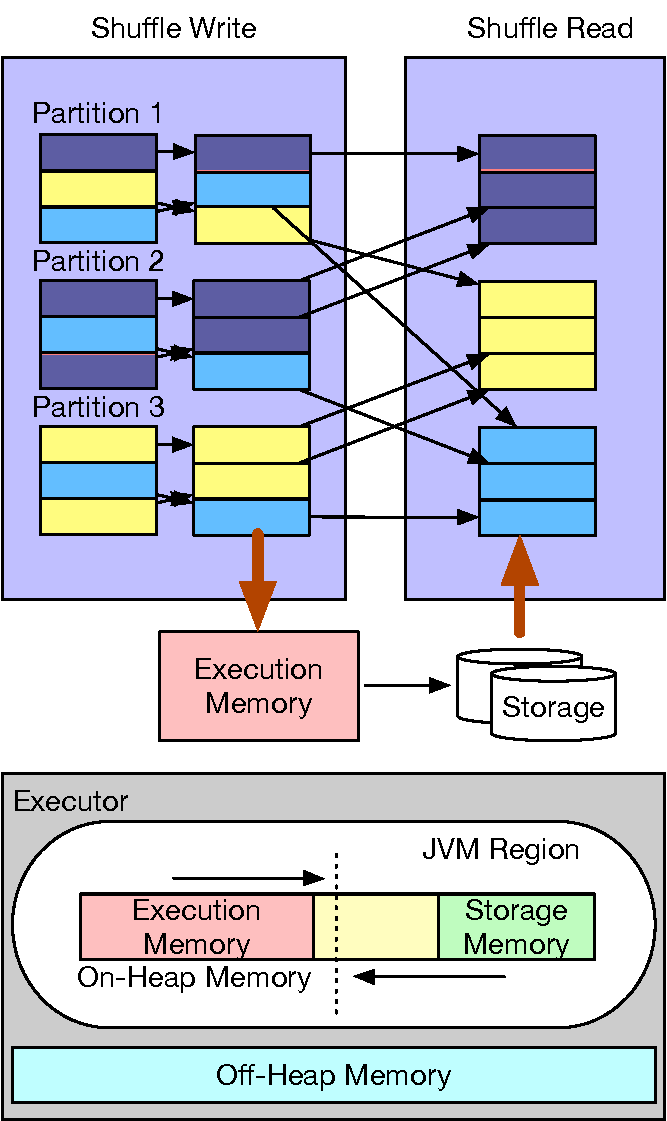
\includegraphics[width=0.5\columnwidth]{fig/cxl/spark.pdf}
  \caption[Spark memory layout and shuffle spill]{\textbf{Spark memory layout and shuffle spill.} Each Spark executor possesses a fixed-size On-Heap memory, which is dynamically divided between execution and storage memory. If there is insufficient memory during shuffle operations, the Spark executor will spill the data to the disk.}
\label{fig:eval_spark_0}
%\vspace{-2.5em}
\end{figure}
Big Data plays a crucial role in the workloads managed by data centers. Due to the scale of data involved in Big Data analytical applications, memory capacity often becomes a bottleneck to the performance~\cite{sparkmemory}. Take Spark~\cite{spark}, one of the common Big Data platforms, as an example: A typical query requires shuffling data from multiple tables for processing in the next stage. Operations like \textit{reduceByKey()} first partition the data according to the key and then execute reduce operators on each key. Such shuffling operation involves disk I/O and network communication between multiple nodes, posing significant overhead on the query. In some cases, the performance of shuffling could dominate the performance of the workload~\cite{PSACS}. During the shuffling process(Fig. \ref{fig:eval_spark_0}), memory usage could grow beyond the capacity or certain threshold (e.g. \texttt{spark.shuffle.memoryFraction}). When this happens, Spark can be configured to spill data to disk to avoid the risk of out-of-memory failure. Since disk I/O is of magnitudes slower than memory, this could significantly impact the workload's performance.

\begin{figure*}[t]
\centering
 %\vspace{-0.2em}
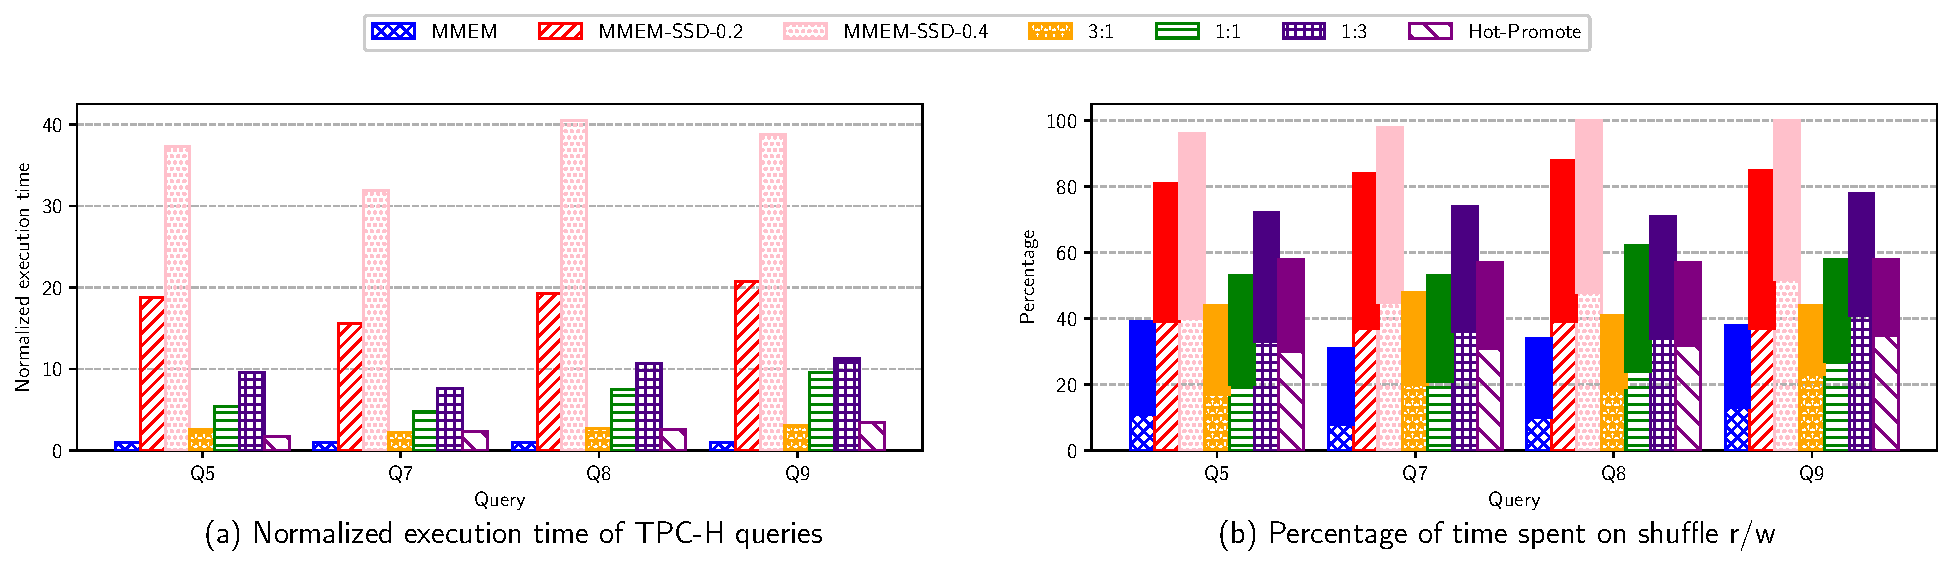
\includegraphics[width=1\textwidth]{fig/cxl/spark_cxl.pdf}
  \caption[Spark execution time and shuffle percentage]{\textbf{Spark execution time and shuffle percentage.} (a) Execution time of each TPC-H query normalized to the execution time running on MMEM. (b) The percentage of time spent of shuffle operation for each query. The solid bars represent shuffle writes, while hollow bars represent shuffle reads.}
\label{fig:eval_spark_1}
\end{figure*}


\subsubsection{Methodology and Software Configurations.}

In our experiment, we aim to test if we could reduce the number of servers needed for a specific workload with minimal effect on overall performance. Therefore, we compared the performance of Spark running TPC-H~\cite{tpch} on three servers without CXL memory expansion vs. on two servers but with CXL memory expansion. We assume the maximum amount of MMEM that could be used on each server is $512$ GB, therefore with three servers, we have $1.5$ TB MMEM and $1$ TB CXL memory in total.
In order to trigger data spill within the workload, we configured $150$ Spark executors. Each Spark executor contains $1$ core and $8$ GB of memory. Therefore the total Spark application occupies $150$ cores and $1.2$ TB of memory. We generate a total of $7$ TB TPC-H initial dataset. We continue to adhere to the configuration settings detailed in Table \ref{tab:swconfig} as follows:
\begin{itemize}
  \item MMEM only: We allocate $50$ Spark executor and $400$ GB on each of the \textbf{three} servers. In this case there is no data spilled to disk as each executor have sufficient amount of memory.
  \item MMEM/CXL interleaving: We distributed the same number of executors ($150$) across the \textbf{two} cxl servers, which has $1$ TB ($512$ GB from each of the two CXL cards) plus $1$ TB of MMEM ($512$ GB each). For example, in a configuration where MMEM and CXL memory usage is balanced (1:1 ratio), we allocated $75$ Spark executors to use $600$ GB MMEM while another $75$ Spark executors to $600$ GB CXL memory. In this case, there is also negligible amount of data spilled to the disk.
  \item Spill to SSD: To simulate conditions where executors would run out of memory and need to spill data to SSD storage, we restrict the memory allocation of the Spark executors to either $80\%$ or $60\%$ of entire $1.2$ TB MMEM. In this case, there will be around $320$ GB and $500$ GB data spilled to the disk respectively.
  \item Hot-Promote: same as prior experiment (\S\ref{ssec:keydb}).
\end{itemize}
We chose four specific queries ($Q5$, $Q7$, $Q8$, and $Q9$) from the TPC-H benchmark~\cite{tpch}, recognized for their intensive data shuffling demands from prior studies~\cite{PSACS}, to evaluate our setup. Importantly, our measurements focused solely on the time to execute these queries, excluding any data preparation or server setup durations. We disabled SNC on all servers.

\subsubsection{Analysis.}
%\yupeng{Maybe change Hot-Promote to hot or sth}

Figure \ref{fig:eval_spark_1} illustrates variations in total execution time across different configurations. To provide a clear comparison, we normalized the total execution time against the best-case scenario, which involves running the entire workload in MMEM. Similar to the KeyDB experiments, the interleaving approach still exhibits a performance slowdown, ranging from $1.4$x to $9.8$x compared to the optimal MMEM-only scenario while using less number of servers. This performance degradation becomes worse as a larger proportion of memory is allocated to CXL. Nevertheless, it's crucial to note that even with this slowdown, the interleaving approach remains significantly faster than spilling data to SSDs. Figure \ref{fig:eval_spark_1}(b) illustrates that shuffling overshadows the total execution time due to the intensification of data spill issues.

A notable difference between the KeyDB and Spark experiments is the performance of HotPromote.
While it performs better in KeyDB, the Spark SQL experiment shows a more than $34\%$ slowdown compared to MMEM.
Unlike the Zipfian distribution in which the hottest keys are moved from CXL to DDR, there is a considerable amount of thrashing behavior within the kernel in the Spark SQL tests.
We identify the root cause after thoroughly investigating the kernel patch implementation.
In the initial version of the hot page selection patch~\cite{hot}, a sysctl knob  "\texttt{kernel.numa\_balancing\_promote\_rate\_limit\_MBps}" is used to control the maximum promoting/demoting throughput.
Subsequent versions introduced an automatic threshold adjustment feature to this patch, aiming to strike a balance between the speed of promotion and migration costs. Nevertheless, this automatic adjustment mechanism appears to fall short in our Spark SQL evaluations. The TPC-H workload on Spark, which demonstrates reduced data locality, challenges the kernel's efficiency in promoting frequently accessed pages. This finding aligns with similar issues highlighted in prior research~\cite{demystify}.

\subsubsection{Insights.}
Our research indicates that utilizing CXL memory expansion offers a cost-efficient approach for data-center applications. We postpone our detailed theoretical examination of the Abstract Cost Model to \S\ref{sec:cost}. Concurrently, although the hot-promote patch demonstrates significant advantages in key-value store workloads, its performance is notably lacking in Spark experiments. As system developers begin to enhance software support for CXL within the kernel, it is crucial to proceed with caution. System-wide policies can have varied impacts on applications, depending on their unique characteristics.

\subsection{Spare Cores for Virtual Machine}

\begin{table*}[!]
  \centering
  % \vspace{-0.5em}
  %\bgroup
  \small
  %\def\arraystretch{0.95}%
  \begin{tabular}{c|c|c|c|c|c} 
        \hline
        Year & CPU & Max vCPU  & Memory channels & Max memory & Required Memory \\
        & & per server & per socket & \textbackslash TB & ($1:4$) \textbackslash TB\\\hline
        $2021$ & IceLake-SP\cite{icelakecores} & $160$ & 8xDDR4-3200 & $4$ & $0.64$ \\\hline
        $2022$ (delayed) & Sapphire Rapids\cite{sprcores} & $192$ & 8xDDR5-4800 & 	$4$ & $0.768$ \\\hline
        $2023$ (delayed) & Emerald Rapids\cite{emeraldrapidscores} & $256$ & 8xDDR5-6400 & $4$ & $1$ \\\hline
        $2024$+  & Sierra Forest\cite{sierraforestcores} & $1152$ & $12$ & $4$ & $4.5$ \\\hline
        $2025$+ & Clearwater Forest\cite{clearwatercores} & $1152$ & TBD & $4$ & $4.5$ \\\hline
  \end{tabular}
  %\egroup
  % \vspace{-0.1em}
  \caption[Intel Processor Series]{\textbf{Intel Processor Series.} }
  \label{tab:amd}
  \vspace{-1.5em}
\end{table*}

One widely-used application within Infrastructure-as-a-Service (IAAS) is Elastic Computing~\cite{elasticcomputing}. Here, cloud service providers (CSPs) offer computational resources to users through virtual machines or container instances. Given the diverse needs of users, CSPs traditionally offer a variety of instance types, each characterized by different configurations of CPU cores, memory, disk, and network capacities. Generally, an "optimal" CPU-to-memory ratio, often cited as 1:4, is employed to balance computational and memory requirements (as per AWS guidelines~\cite{awsm7a, awsm7i}). For example, an instance with $128$ vCPUs would typically feature $512$ GB of DDR memory.
Advancements in server processor architecture and chiplet technology have spurred rapid increases in the number of cores available in a single processor package, driven in large part by the CSPs' aim to lower per-core costs. Consequently, 2-socket servers have seen their vCPU counts grow from $160$ to $256$ within the past two years (Table~\ref{tab:amd}). This trend is projected to continue, reaching as many as $1152$ vCPUs per server by $2025$.


The surge in vCPUs exacerbates memory capacity bottlenecks, constrained by DDR slot limits, DRAM density, and the cost of high-density DIMMs. Intel's Sierra Forest Xeon, for example, supports $1152$ vCPUs but is limited by motherboard design to less than $4$ TB of memory, falling short of the typical $4.5$ TB needed for VM provisioning~\cite{1dpc}. This discrepancy makes maintaining a cost-effective vCPU-to-memory ratio challenging, resulting in underutilized vCPUs and lost revenue for CSPs. CXL memory expansion provides a solution by enabling memory capacity to scale beyond DDR limitations, ensuring optimal vCPU utilization and mitigating revenue losses for CSPs.

\subsubsection{Methodology and Software Configurations.}

To assess the performance impact when an application operates exclusively on CXL memory, we replicate the KeyDB configuration from previous experiments (\S\ref{ssec:keydb}). We utilize \textit{numactl} to allocate the KeyDB instance exclusively to MMEM or CXL memory. For our evaluation, the workload employed is YCSB-C, characterized by $1$ KB key-value pairs and a total dataset size of $100$ GB. SNC is disabled.

\subsubsection{Analysis.}
The CDF of read latency (Fig. \ref{fig:eval_vm_0}) indicates that applications running on CXL experience a latency penalty of $9\%-27\%$ which is less than the raw data fetching numbers in our previous measurements in \S\ref{sec:micro}. This is due to the processing latency within Redis. The throughput of running the entire workload on CXL memory is around $12.5\%$ less compared to MMEM as show in Fig. \ref{fig:eval_vm_1}.

Now consider a server operating at a sub-optimal vCPU-to-memory ratio of 1:3:
(1) Due to inadequate memory, only $75\%$ of the vCPUs can be sold at the optimal 1:4 ratio, resulting in a $25\%$ revenue loss. Implementing CXL memory expansion enables the CSP to sell the remaining $25\%$ of vCPUs at the optimal ratio.
(2) Our benchmarks indicate that instances running on CXL memory perform $12.5\%$ slower than those on DDR for common workloads such as Redis. Assuming a $20\%$ price discount on such instances, CSPs could still recover approximately $80\%$ of the lost revenue, equating to a ~$27\%$ improvement in total revenue ($20/75 = 26.77\%$).

\begin{figure}[t]
\centering
% \vspace{-0.2em}
\begin{minipage}{0.47\columnwidth}
  \centering
  \subfigure[CDF of KeyDB YCSB-C]{
    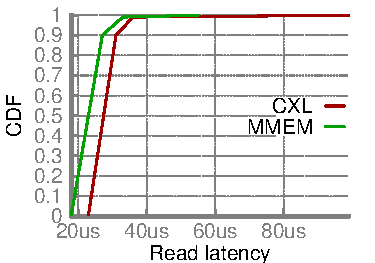
\includegraphics[width=\textwidth]{fig/cxl/new_read_latency_cdf.pdf}
    \label{fig:eval_vm_0}
  }
\end{minipage}\hfill
\begin{minipage}{0.53\columnwidth}
  \centering
  \subfigure[Throughput of KeyDB YCSB-C]{
    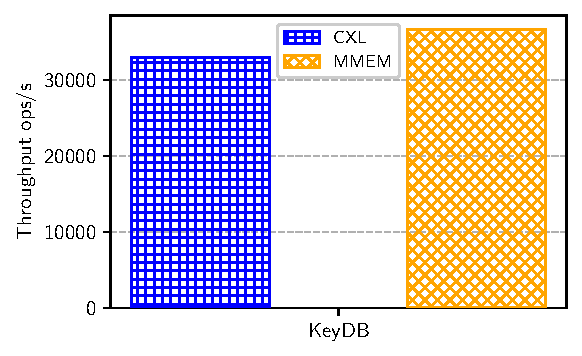
\includegraphics[width=\textwidth]{fig/cxl/redis_ycsb.pdf}
    \label{fig:eval_vm_1}
  }
\end{minipage}
\caption[KeyDB Performance with YCSB-C on CXL/MMEM]{\textbf{KeyDB Performance with YCSB-C on CXL/MMEM.}}
\vspace{-1.5em}
\end{figure}

\subsubsection{Insights.}
Given the sheer scale of Elastic Computing Service (ECS) applications in public clouds, the potential benefits of CXL memory expansion could be substantial. However, the challenge of maintaining an optimal virtual CPU (vCPU) to memory ratio, traditionally at 1:4, becomes more complex with the rapid increase in processor cores. This ratio, although standard, is under scrutiny for its applicability in future cloud computing paradigms. Notably, Bytedance's Volcano Engine Cloud ~\cite{volcano} illustrates the variability in resource allocation by offering different ratios: 1:4 for general purposes, 1:2 for compute-intensive tasks, and 1:8 for memory and storage-intensive workloads. The impact of CXL memory expansion and pooling on these established ratios presents an intriguing avenue for exploration, raising questions about the adaptability of cloud providers to evolving hardware capabilities and the subsequent effect on resource allocation standards.




\section{Memory Bandwidth-Bound applications}

\label{sec:bandwidth}

The other advantage of CXL memory expansion is its extra memory bandwidth. We use Large Language Model inference as an example to showcase how this can benefit real-world applications.

Recent work on LLM~\cite{gpt4} shows that LLM inference is hungry for memory capacity and bandwidth.
The limited capacity of GPU memory restricts the batch size of the LLM inference job and reduces computing efficiency since LLM models are memory-demanding.
On the other hand, while CPU memory is high in capacity, it has lower bandwidth than GPU memory.
The extra bandwidth and capacity offered by CXL memory make it a promising option for alleviating this bottleneck.
For example, a CPU-based LLM inference job can benefit from the extra bandwidth brought by CXL memory, and a CXL-enabled GPU device can also use the extra memory capacity from a disaggregated memory pool.
Due to the lack of CXL support in current GPU devices, we experiment with LLM inference on CPU to study the implications of CXL memory's extra bandwidth.
We also note that as LLM inference applications are agnostic to the underlying memory technologies, the findings and implications from our experiments are also applicable to the upcoming CXL 2.0/3.0 devices.


\begin{figure}[t]
\centering
 %\vspace{-0.2em}
 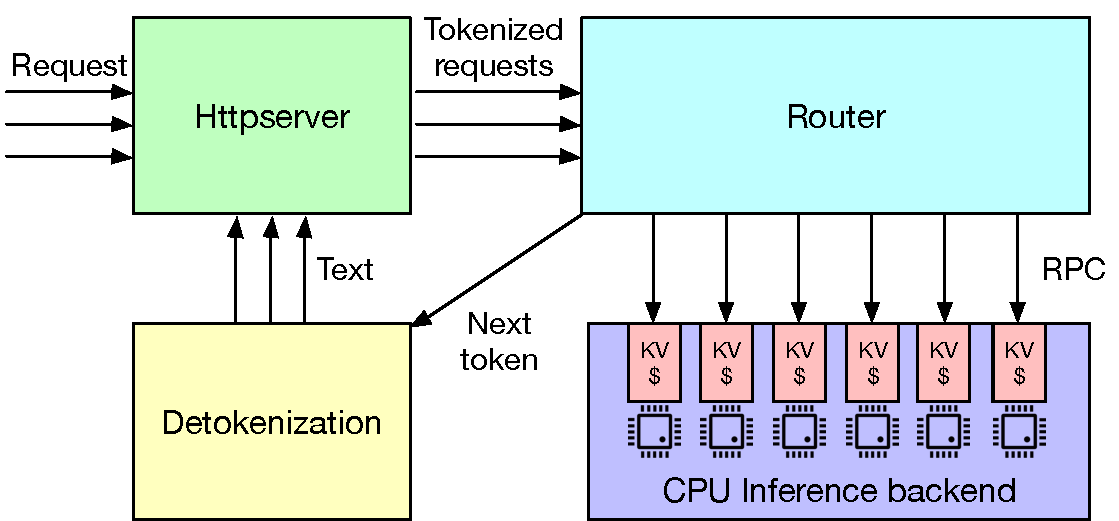
\includegraphics[width=\columnwidth]{fig/cxl/llm.pdf}
  \caption[LLM inference framework]{\textbf{LLM inference framework.} The Httpserver receive requests and forward the tokenized requests to the CPU inference backend. The CPU inference backend serves the requests and reply the next token.}
\label{fig:llm-framework}
\vspace{-2.5em}
\end{figure}

\begin{figure*}[h!]
\centering
% \vspace{-0.2em}
\subfigure[LLM inference serving rate vs. number of threads]{
  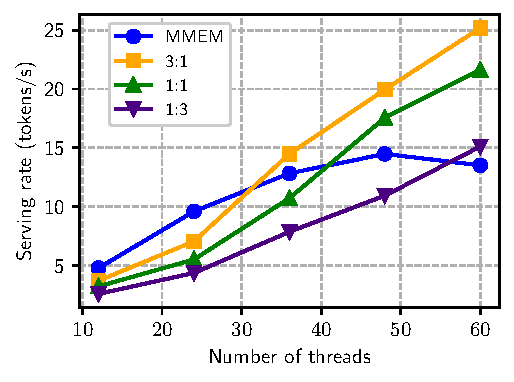
\includegraphics[width=0.31\textwidth]{fig/cxl/llm_serving.pdf}
  \label{fig:eval-llm-1}
}
\subfigure[Memory bandwidth vs. number of threads for a single backend]{
  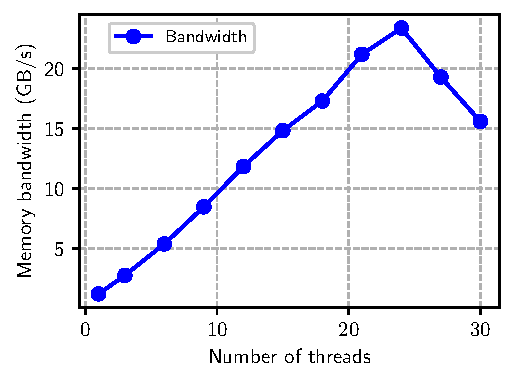
\includegraphics[width=0.31\textwidth]{fig/cxl/llm_bandwidth.pdf}
  \label{fig:eval-llm-2}
}
\subfigure[Memory bandwidth vs. KVcache size for a single backend]{
  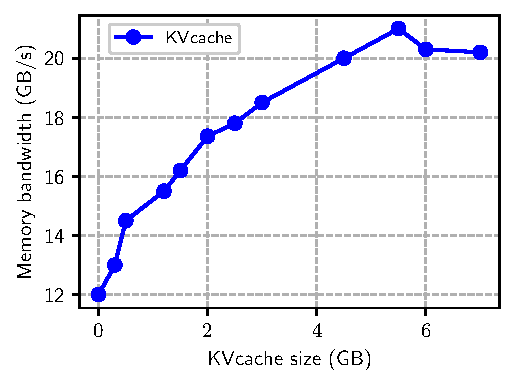
\includegraphics[width=0.31\textwidth]{fig/cxl/kvcache.pdf}
  \label{fig:eval-llm-3}
}
\vspace{-0.5em}
\caption[CPU LLM inference]{\textbf{CPU LLM inference.} }
\vspace{-0.5em}
\end{figure*}

\paragraphb{LLM Inference Framework}
Mainstream Large Language Model (LLM) inference frameworks, such as vLLM~\cite{vllm} and LightLLM~\cite{lightllm}, do not support CPU inference. Recently, Intel introduced an LLM model named Q8chat~\cite{q8chat}, trained using their 4th Generation Intel Xeon® Scalable Processors. However, the inference code for Q8chat is not yet publicly available. 
To address this gap, we have developed our inference framework based on the open-source LightLLM framework~\cite{lightllm} by replacing the backend with a CPU inference backend. Figure~\ref{fig:llm-framework} illustrates our implementation.
In our framework, the HTTPserver frontend receives LLM inference requests and forwards the tokenized requests to a router. The router is responsible for distributing these requests to different CPU backend instances. Each CPU backend instance is equipped with a Key-Value (KV) cache~\cite{kvcache}, a widely used technique in large language model inference. It's worth noting that KV caching, despite its name, differs from the traditional 'key-value store' in system architecture. KV caching occurs during multiple token generation steps, specifically within the decoder. During the decoding process, the model starts with a sequence of tokens, predicts the next token, appends it to the input, and repeats this generation process. This is how models like GPT~\cite{gpt4} generate responses. The KV cache stores key and value projections used as intermediate data within this decoding process to avoid recomputation for each token generation. Prior research~\cite{kvcache} has shown that KV caching is typically memory-bandwidth bound, as it is unique for each sequence in the batch, and different requests typically do not share the KV cache since the sequences are stored in separate contiguous memory spaces~\cite{vllmpaper}.


\subsection{Methodology and Software Configurations}
To investigate the benefits of CXL memory extension for applications with high memory bandwidth demands and limited MMEM bandwidth availability, we employ the SNC-4 configuration to divide a single CPU into four sub-NUMA nodes. Each node is equipped with two DDR5-4800 memory channels, facilitating an early memory bandwidth saturation of $67$ GB/s (\S\ref{sec:micro}). We examine three distinct interleaving policies ($3$:$1$, $1$:$1$, $1$:$3$), detailed in Table \ref{tab:swconfig}. The CPU inference backend is configured with 12 CPU threads, and memory allocation is strictly bound to a single sub-NUMA domain. This domain includes two DDR5-4800 channels and a $256$ GB A1000 CXL memory expansion module via PCIe. By binding allocations to a single node, we ensure the initial saturation of the DDR5 channels. Our experiments utilize the Alpaca 7B model~\cite{alpaca}, an advancement of the LLaMA 7B model, requiring 4.1GB of memory. The workload, derived from the LightLLM framework~\cite{lightllm}, includes a wide range of chat-oriented questions. A single-threaded client machine on a baseline server sends HTTP requests with various LLM queries to mimic real-world conditions. The client ensures continuous operation of the CPU inference backends by maintaining a constant stream of requests. The prompt context is set to 2048 bytes to guarantee a minimum inference response size. We progressively increase the CPU inference backend count to monitor the LLM inference serving rate (in tokens/s).

\subsection{Analysis}
Fig. ~\ref{fig:eval-llm-1} displays the inference serving rates across various memory configurations as the thread count, i.e., the number of CPU inference backends, increases. Initially, the serving rate improves almost linearly with available memory bandwidth. However, at $48$ threads, MMEM bandwidth saturation limits the serving rate, whereas the interleaving configurations leverage additional CXL bandwidth for continued scaling. With a significant number of inference threads ($60$), an MMEM:CXL = $3$:$1$ interleaving significantly surpasses the MMEM-only approach by $95\%$.

Interestingly, among the interleaving policies, configurations with a higher proportion of data in main memory demonstrate superior inference performance. Contrary to expectations, we observe that operating entirely on main memory is $14\%$ less effective than a MMEM:CXL ratio of $1$:$3$ beyond $64$ threads. This outcome is notable given CXL's inherently higher latency and reduced memory bandwidth (\S~\ref{sec:micro}). Fig. \ref{fig:eval-llm-2} charts the memory bandwidth utilization, as measured by the Intel Performance Counter Monitor (PCM) \cite{pcm}, with increasing CPU thread counts within a single CPU inference backend. Initially, bandwidth utilization grows linearly with thread count, plateauing at $24.2$ GB/s for $24$ threads. This trend allows us to estimate a bandwidth of approximately $63$ GB/s at $60$ threads, reaching $82\%$ of the theoretical maximum. Our microbenchmark findings, as detailed in \S\ref{sec:micro}, indicate that this level of bandwidth utilization may lead to significant latency spikes. These results corroborate the hypothesis that bandwidth contention plays a crucial role in the observed performance degradation.

Bandwidth contention may stem from either loading the LLM model or accessing the KV cache. Adjusting the prompt context to infinity enables the LLM model to continuously generate new tokens for storage in the KV cache. Fig. ~\ref{fig:eval-llm-3} illustrates the correlation between KV cache size and memory bandwidth consumption. The initial memory bandwidth of approximately $12$ GB/s originates from I/O threads loading the model from memory. When storing information for a larger sequence of tokens in the KV cache, memory usage initially increases linearly. However, bandwidth utilization stops increasing beyond roughly $21$ GB/s. 

\subsection{Insights}
Interestingly, existing tiered memory management in the kernel does not consider memory bandwidth contention. Considering a workload that uses high main memory bandwidth(e.g., $70\%$), existing page migration policy(\S\ref{sec:background}) tends to move data from slower tiered-memory (CXL) into MMEM, supposing that there is still enough memory capacity. As more data is written into the main memory, the memory bandwidth will continue to increase (e.g., $90\%$). In this case, the access latency will grow exponentially, resulting in an actual slowdown of the workload. This scenario will not be uncommon, especially for memory-bandwidth-bound applications (e.g., LLM inference). Therefore, the definition of tiered memory requires rethinking.










% !TEX root = ../paper.tex

\section{Cost Implications}
% \yupeng{This section name is subject to change.}
\label{sec:cost}
\begin{table}[btp!]
  \centering
  \footnotesize
  \begin{tabular}{l|l}
    \hline
    Parameter & Description \\ \hline
    $P_s$  & \makecell[l]{Throughput when (almost) entire working set is spilled to SSD on a server. \\ Normalized to 1 in the cost model.}  \\  \hline
    $R_d$ & \makecell[l]{Relative throughput when the entire working set is in main memory on a server, normalized to $P_s$.}   \\ \hline
    $R_c$ & \makecell[l]{Relative throughput when the entire working set is in CXL memory on a server, normalized to $P_s$.}  \\ \hline
    $D$ & \makecell[l]{The MMEM capacity allocated to each server. For completeness only, not used in cost model.} \\ \hline
    $C$ & \makecell[l]{The ratio of main memory to CXL capacity on a CXL server. \\ E.g. 2 means the server has 2x MMEM capacity than CXL memory.} \\ \hline
    $N_{baseline}$ & Number of servers in the baseline cluster. \\ \hline
    $N_{cxl}$ & \makecell[l]{Number of servers in the cluster with CXL memory to deliver the same performance as the baseline.} \\ \hline
    $R_t$ & \makecell[l]{Relative TCO comparing a server equipped with CXL memory vs. baseline server. \\ E.g. If a server with CXL memory costs $10\%$ more than the baseline server, this parameter is $1.1$.} \\ \hline 
  \end{tabular}
  \caption[Parameters of our Abstract Cost Model]{\textbf{Parameters of our Abstract Cost Model.}}
  \label{tab:roi}
\end{table}


Our comprehensive analysis in prior sections (\S\ref{sec:capacity}, \S\ref{sec:bandwidth}) reveals that the adoption of CXL memory expansion offers substantial benefits for data center applications, including comparable performance with operational cost savings. However, a significant hurdle in embracing such innovative technology as CXL lies in determining its Return on Investment (ROI). Despite having access to detailed technical specifications and benchmark performance results, accurately forecasting the Total Cost of Ownership (TCO) savings remains challenging. The complexity of simulating benchmarks at production scale, compounded by the limited availability of CXL hardware, exacerbates this issue. Traditional cost models in prior work~\cite{CXLPoolCost}, which could offer such forecasts, demand extensive internal and sensitive information that is often inaccessible. To overcome this barrier, we propose an Abstract Cost Model designed to estimate TCO savings independently of internal or sensitive data. This model leverages a select set of metrics obtainable through microbenchmarks, alongside a handful of empirical values that are simpler to approximate or access, providing a viable means to evaluate the economic viability of CXL technology implementation.

We use a capacity-bound application (Spark SQL) as an example to demonstrate how we develop our Abstract Cost Model, but our methodology can be extended to other types of workloads as well. For Spark SQL applications, the additional capacity enabled by CXL memory reduces the amount of data spilled to SSD and results in higher performance (throughput).
This means fewer servers will be needed to meet the same performance target.

Given that the workload maintains a relatively consistent memory footprint (the size of the active dataset) during execution, we can approximate the execution time of the workload by dividing it into three distinct segments: (1) The segment processed using data stored in MMEM, (2) The segment processed using data stored in CXL memory, and (3) The segment processed using data that has been offloaded to SSD storage.


We first make these measurements from microbenchmarks on a single server:
\begin{itemize}
  \item Baseline performance ($P_s$):
  % \HX{dataset spilled to SSD is under the context of SparkSQL, which is bandwidth related not capacity related, correct? This section is "Capacity bound applications".}
  Measure the throughput when (almost) all working set is spilled to SSD. The absolute number is not used in our cost model. Instead, we then normalize it to 1 in our cost model.
  \item Relative performance when the entire working set is in MMEM ($R_d$): Using the same workload, we measure the throughput when the entire working set is in MMEM and normalize it to $P_s$ to get the relative performance (i.e., how much faster compared to the baseline).
  \item Relative performance when the entire working set is in CXL memory ($R_c$): Using the same workload, we measure the throughput when the entire working set is in CXL memory, and normalize it to $P_s$ to get the relative performance.
\end{itemize}

We then formulate our cost model using the parameters outlined in Table~\ref{tab:roi}. For a working set size of $W$, the execution time of the baseline cluster could be approximated as the sum of two segments:
1) the segment that is executed with data in MMEM; 2) the segment that is executed with data spilled onto SSD.

% Assuming the Workload working set size is $ W $, with a part running in DRAM and a part spilling to SSD, the running time for the baseline cluster is:

$$
T_{baseline} = \frac{N_{baseline} D}{R_d} + (W - N_{baseline}D)
$$

The execution time of the cluster with CXL memory could be approximated in a similar way.
It includes the segment that is executed with data in main memory, in CXL memory, and spilled to SSD respectively.

$$ T_{cxl} = \frac{N_{cxl} D}{R_d} + \frac{N_{cxl} D}{CR_c} + (W - N_{cxl} D - \frac{N_{cxl} D}{C}) $$

To meet the same performance target, $T_{baseline} = T_{cxl}$:

% Under the same SLA conditions, $ T1 = T2 $, thus:

$$
\frac{N_{baseline} D}{R_d} - N_{baseline} D = \frac{N_{cxl} D}{R_d} + \frac{N_{cxl} D}{CR_c} - N_{cxl} D - \frac{N_{cxl} D }{C}
$$

% After some simple transformations, we have:

% $$ (C+1)/C - (C R_c + R_d) / (C R_c R_d) N_{cxl} = (R_d - 1) / R_d N_{baseline} $$

With some simple transformations, we get the ratio between $N_{cxl}$ and $N_{baseline}$: 
% Comparing the sizes of baseline and CXL clusters, we have:

$$ \frac{N_{cxl}}{N_{baseline}} = \frac{CR_c(R_d - 1)}{R_cR_d(C+1) - C R_c - R_d} $$

TCO saving can then be formulated as follows.

$$
TCO_{saving}=1-\frac{TCO_{cxl}}{TCO_{baseline}}=1-\frac{N_{cxl} R_t}{N_{baseline}}
$$

% \yupeng{TODO: change these numbers}
% Using our Redis experiments(\S\ref{sec:capacity}) as an example, we measure that

For example, suppose $ R_d = 10 $, $R_c = 8 $, $ C = 2 $, we get $\frac{N_{cxl}}{N_{baseline}} = 67.29\%$ from the cost model.
This means that by using CXL memory, we may reduce the number of servers by $32.71\%$.
And if we further assume $R_t=1.1$ (a server with CXL memory costs $10\%$ more than the baseline server), the TCO saving is estimated to be $25.98\%$.

Our Abstract Cost Model provides an easy and accessible way to estimate the benefit from using CXL memory,
providing important guidance to the design of the next-generation infrastructure.

\paragraphb{Extending Cost Model for more realistic scenarios}
In line with previous research \cite{CXLPoolCost}, our Abstract Cost Model is designed to be adaptable, allowing for the inclusion of additional practical infrastructure expenses such as the cost of CXL memory controllers, CXL switches (applicable in CXL 2.0/3.0 versions), PCBs, cables, etc., as fixed constants. However, a notable constraint of our current model is its focus on only one type of application at a time. This becomes a challenge when a data center provider seeks to evaluate cost savings for multiple distinct applications, each with unique characteristics, especially in environments where resources are shared (for instance, through CXL memory pools). This scenario introduces complexity and presents an intriguing challenge, which we acknowledge as an area for future investigation.

% \subsection{Bandwidth bound applications}